\documentclass{article}
\usepackage[a4paper, left=2mm, right=2mm, top=5mm, bottom=5mm]{geometry}
\usepackage[pdftex]{graphicx}
\usepackage{ucs}
\usepackage{tikz}
\usepackage{pgfplots}
\pgfplotsset{compat=1.9}
\usepackage{pgfplots}
\usepackage[utf8x]{inputenc} % Включаем поддержку UTF8  
\usepackage[russian]{babel}  % Включаем пакет для поддержки русского языка 
\graphicspath{{/}}
\linespread{2}
\DeclareGraphicsExtensions{.jpg}
\begin{document}

\includegraphics[width=2.4cm]{mirea} 
\begin{center}
\begin{LARGE}
\textbf{Московский государственный технический университет}\\
\textbf{радиотехники, электроники и автоматики}\\
\textbf{(МГТУ МИРЭА)} \\
~\\
\hrule \vspace {10pt}
\textbf{Институт высоких технологий} \\

\textbf{Кафедра «Теплофизические приборы и аппараты»} \\
Дисциплина (модуль) \textbf{«Информационные технологии\\
в АКТ»} \\
\end{LARGE}
\begin{Huge}
\textbf{Курсовая Работа}\\
\end{Huge}
\begin{large}
Тема: 
\end{large}
\begin{normalsize}
“Расчет параметров двигателя на квазистационарных режимах” \\
\end{normalsize}
~\\
~\\
\begin{large}
Вариант №4\\

\end{large}
\end{center}
\begin{flushright}
Выполнил студент группы ВТ7 - 1201\\
\rule{4cm}{0.01pt} / А.Л. Чукаева / \\
~\\
\end{flushright}
\begin{flushleft}
Отметка о защите \rule{5cm}{0.01pt} \\
\end{flushleft}
\begin{flushright}

Преподаватель каф. ВТ-7 \\
\rule{4cm}{0.01pt} / В.В. Кадомкин / \\
~\\
~\\
\end{flushright}
\begin{center}
\textbf{Москва - 2015}
\end{center}

\begin{flushright}
\begin{scriptsize}
\textit{160700.65   Проектирование авиационных и ракетных двигателей\\
 Информационные технологии в АКТ: Лабораторный практикум} \\
 \end{scriptsize}
\end{flushright}
\begin{center}
\textbf{Курсовая работа}\\
\end{center}
~\\
\textbf{\textit{Тема:}}
Расчет параметров двигателя на квазистационарных режимах\\
~\\
\textbf{\textit{Цель работы:}}
В данной работе выполняется расчет на ПЭВМ параметров рабочих процессов двигателя с заданной начальной формой заряда. По результатам расчетов определяется изменение во площади поверхности горения, давление в камере сгорания, параметры потока по длине сопла и изменение тяги двигателя во время работы РДТТ.
\begin{center}
\textbf{\textit{Общие положения и теоретические сведения}}

\end{center}
На стационарном режиме работы РДТТ в каждый момент времени устанавливается баланс между приходом продуктов сгорания от твердого топлива и расходом продуктов сгорания через сопло. Учитывая, что поверхность горения заряда ТТ (в общем случае) не остается величиной постоянной, то баланс массы для продуктов сгорания в газовом объеме КС должен описываться дифференциальным уравнением вида
\begin{equation}\label{eq:fourierrow} 
\frac{dm}{dt}= \frac{d(\rho V_k)}{dt} = P_T - G_c
\end{equation}\\
где масса продуктов сгорания в КС, плотность продуктов сгорания, свободный объем камеры сгорания, секундный массовый приход продуктов приходом продуктов сгорания от твердого топлива, расход продуктов через выходное сопло.\\
При запуске двигателя давление в камере сгорания постепенно нарастает до тех пор, пока не достигнет некоторого заданного уровня, что эквивалентно накоплению массы газа и энергии в газовой зоне камеры сгорания. Приход продуктов при запуске двигателя превышает расход продуктов сгорания через сопло и этому, в частности, способствует дополнительный приход продуктов сгорания при работе воспламенителя.\\
При выходе на стационарный режим приход и расход продуктов уравновешивают друг друга. Приход и расход продуктов сгорания будет в процессе работы двигателя изменяться в определенных пределах, на характерные времена установления режима в КС часто гораздо меньше характерных времен изменения параметров рабочего процесса. Это относится к основным режимам работы (стационарным или квазистационарным) и должно быть получено соотношение, позволяющее найти параметры для расчета стационарные режимы энергосистем.\\
~\\
Приход продуктов в камере сгорания определяется массой сгоревшего топлива за единицу времени: \\
\begin{equation}\label{eq:fourierrow} 
P_t = V_g * \rho_T 
\end{equation}\\


\begin{flushright}
\begin{scriptsize}
\textit{160700.65   Проектирование авиационных и ракетных двигателей\\
 Информационные технологии в АКТ: Лабораторный практикум} \\
\end{scriptsize}
\end{flushright}
\begin{equation}\label{eq:fourierrow} 
V_g = S_g * u 
\end{equation}
\begin{equation}\label{eq:fourierrow} 
P_t = \rho_T * S_g * u,
\end{equation}
где объем сгоревшего топлива в единицу времени, плотность топлива, скорость горения ТТ.\\
~\\
Скорость химических реакций существенно зависит от давления. Из-за сложного механизма взаимодействия газовой и конденсированной зон, конкурирующих процессов тепло-массопереноса для описания процесса горения твердого топлива часто используют эмпирические законы для скорости горения. В частности, для зависимости скорости горения топлива от давления может быть использован степенной закон для скорости горения:\\
\begin{equation}\label{eq:fourierrow} 
u = u_1 * {(\frac{P_k}{P_1})}^v = u(P_k)
\end{equation}\\
где p1 – некоторый выбранный уровень давления, который является характерным для работы топлива данного типа.\\
В качестве уровня давления могут быть выбраны и стандартные условия для атмосферы, хотя при этих условиях топлива могут не гореть, и выполнятся просто перерасчет имеющихся данных о скорости горения к стандартным условиям. \\
\begin{equation}\label{eq:fourierrow} 
u = u_{10} * {(\frac{P_k}{P_0})}^v = u_1 * {(\frac{P_k}{P_1})}^v
\end{equation}\\
\begin{equation}\label{eq:fourierrow} 
u_{10} = u_1 * {(\frac{P_0}{P_1})}^v
\end{equation}\\
Часто используют приведенные скорости горения к стандартным условиям, но при этом оговаривают диапазон применения соотношений по давлению. Уравнение прихода газа запишем \\
\begin{equation}\label{eq:fourierrow} 
P_T = \rho * S_g *u_1 * {(\frac{P_k}{P_0})}^v
\end{equation}\\
Учитывая, что выходное сопло РДТТ после выхода двигателя на режим работает в режиме критическом или сверхкритическом режиме истечения, то расход продуктов через сопло определяется соотношением: \\
\begin{equation}\label{eq:fourierrow} 
G_{nozzle} = \frac{P_k F_{kr}}{\beta}
\end{equation}\\
где $\beta$ - расходный комплекс (имеет размерность скорости и для топлив принимает значение порядка 1400 – 1800 м/с).


\begin{flushright}
\begin{scriptsize}
\textit{160700.65   Проектирование авиационных и ракетных двигателей\\
 Информационные технологии в АКТ: Лабораторный практикум} \\
 \end{scriptsize}
\end{flushright}
Учитывая, что выполняется баланс между приходом и расходом продуктов, получил
\begin{equation}\label{eq:fourierrow} 
\rho_T * S_g * u_1 * {(\frac{P_k}{P_0})}^v = \frac{P_k * F_{kr}}{\beta}
\end{equation}\\
Из этого уравнения можем найти соотношение для расчета давления в камере сгорания pк, которое позволит по конструктивным параметрам энергосистемы и свойствам топлива найти параметры рабочего процесса на стационарных режимах.\\
Коэффициент в степенном законе горения может изменятся в диапазоне от 0 до 1. Большие значения $\nu$ соответствуют специальным топливам, используемых для в РДТТ с глубоким регулирования двигателя по тяге. Для обычных топлив $\nu$ принимает значения порядка 0,2…0,5.
Выполняем необходимые преобразования в уравнении баланса расхода
\begin{equation}\label{eq:fourierrow} 
P_k^\nu * \frac{\rho_T * S_g * u_1}{P_0^\nu } = \frac{P_k * F_{kr}}{\beta}
\end{equation}\\
\begin{equation}\label{eq:fourierrow} 
P_k^{\nu-1} * \frac{\rho_T * S_g * u_1 * \beta}{F_{kr} * P_0^\nu }
\end{equation}\
и получаем формулу Бори
\begin{equation}\label{eq:fourierrow} 
P_k = {(\frac{\rho_T * S_g * u_1 * \beta}{F_{kr} * P_0^\nu})}^{\frac{1}{1 - \nu}}
\end{equation}\\
Данное соотношение используется для определения основных параметров двигателя на расчетных режимах, для анализа возможностей регулирования двигателя, анализа возможных изменений параметров при нештатных режимах работы, оценок изменения параметров рабочих процессов в зависимости от технологических разбросов, по мере разгара критического сечения сопла и т.д..\\
\begin{center}
\textbf{\textit{Данные варианта:}}\\
~\\
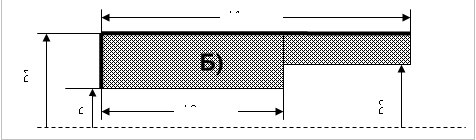
\includegraphics[width=7.4cm]{1} \\
\end{center}
\begin{flushright}
{\textit{Рис. №1: Форма заряда по варианту}}\\
\end{flushright}
\begin{center}
\begin{tabular}{  | c | c | c | c | }
\hline
N1 & N2 & N3 & N4 \\
\hline
Б & A & В & A \\
\hline
\end{tabular}
\end{center}
~\\
\begin{flushright}
\begin{scriptsize}
\textit{160700.65   Проектирование авиационных и ракетных двигателей\\
 Информационные технологии в АКТ: Лабораторный практикум} \\
 \end{scriptsize}
\end{flushright}
\begin{center}
\textbf{\textit{Исходные данные}}\\
\end{center}
\begin{flushright}
\textit{Таблица №2: Исходные данные}\\
\end{flushright}
~\\
\begin{center}
\begin{tabular}{  | c | c | c | c | c | c | c | }
\hline
Parameter & Value & Dimension & Index & Designation & Size & SI \\
\hline
\multicolumn{6}{|c}{Dimensions charge} & \\
\hline
Length & 1.500000 & m & 1 & L10 & 1.500000 & m \\
  & 1 & m & 1 & L20 & 1 & m \\
\hline
Diam & 0.500000 & m & 1 & D10 & 0.500000 & m \\
  & 0.250000 & m & 1 & D20 & 0.250000 & m \\
  & 0.300000 & m & 1 & D30 & 0.300000 & m \\
\hline
\multicolumn{6}{|c}{Data on fuel and combustion products} & \\
\hline
The burning rate & 2 & mm/s & 0 & u & 0.002500 & m/s \\
\hline
The index rate & 0.250000 &  -  & 1 & $\nu$ & 0.250000 &  -  \\
\hline
The base pressure for the unit speed & 100000 & Pascal & 1 & $P_0$ & 100000 & Pascal \\
\hline
Indicator isentrope combustion & 1.220000 &  -  & 1 & k & 1.220000 &  -  \\
\hline
Calculated value of the pressure in the CC & 14 & MPascal & 1000000 & $P_k$ & 14000000 & Pascal \\
\hline
Estimated value of the pressure at the nozzle exit & 20 & kPascal & 1000 & $P_a$ & 20000 & Pascal \\
\hline
The temperature in the combustion chamber & 3200 & K & 1 & $T_k$ & 3200 & K \\
\hline
Molar Mass & 34 & mole & 1 & $\mu$ & 34 & mole \\
\hline
The specific gas constant &  &  &  & $R_{spec}$ & 244.529412 & J/(kg*K) \\
\hline
Fuel Density & 1650 & kg/$m^3$ & 1 & $\rho$ & 1650 & kg/$m^3$ \\
\hline
The time step & 0.120000 &  -  & 1 & h & 0.120000 &   \\
\hline
Consumables complex &  &  &  & $\beta$ & 1497.668067 &   \\
\hline
Critical speed of sound &  &  &  & $A_{kr}$ & 927.382650 &   \\
\hline
Throat area &  &  &  & $F_{kr}$ & 0.002322 & $m^2$ \\
\hline
The diameter of the critical cross-section &  &  &  & $D_{kr}$ & 0.054371 &   \\
\hline
\multicolumn{6}{|c}{Data on fuel and combustion products} & \\
\hline
Angle & 75 & grade &  & $\phi_1$ & 1.308997 & radians \\
\hline
\multicolumn{6}{|c}{The geometry of the supersonic part of the nozzle: conical} & \\
\hline
Angle & 20 & grade &  & $\phi_2$ & 0.349066 & radians \\
\hline
\end{tabular}
\begin{flushright}
\begin{scriptsize}
\textit{160700.65   Проектирование авиационных и ракетных двигателей\\
 Информационные технологии в АКТ: Лабораторный практикум} \\
\end{scriptsize}
\end{flushright}
\begin{center}
\textbf{\textit{The calculated data}}\\
\end{center}
\begin{flushright}
\textit{Table $N^o 3$: The calculated data}\\
\end{flushright}
\begin{tabular}{  | c | p{1.5cm} | p{1.5cm} | p{1.5cm} | c | c | p{1.5cm} | }
\hline
The diameter at the nozzle exit &  &  &  & $D_a$ & 0.305840 & m \\
\hline
Cross-sectional area at the nozzle exit &  &  &  & $F_a$ & 0.073462 & $m^2$ \\
\hline
Area ratio &  &  &  & Fkr/Fa & 0.031604 & - \\
\hline
Maximum dimensionless speed &  &  &  & $\lambda_{max}$ & 3.176619 & - \\
\hline
The dimensionless speed &  &  &  & $\lambda$ & 2.703413 & - \\
\hline
Speed at the nozzle exit &  &  &  & $\nu_a$ & 2507.098360 & - \\
\hline
Gas-dynamic functions &  &  &  & $\pi(\lambda$) & 0.000789 & - \\
\hline
Gas-dynamic functions &  &  &  & $\varepsilon(\lambda$) & 0.002863 & - \\
\hline
Gas-dynamic functions &  &  &  & q($\lambda$) & 0.012438 & - \\
\hline
The difference to the PI(lambda * a) - Pa / Pk &  &  &  &  & -0.000639 & - \\
\hline
The difference to the qu(lambda * a) - Fkr / Fa &  &  &  &  & -0.019166 & - \\
\hline
The length of the subsonic part of the nozzle &  &  &  & $L_{bpn}$ & 0.059703 & m \\
\hline
The length of the supersonic part of the nozzle &  &  &  & $L_{apn}$ & 0.345453 & m  \\
\hline
\end{tabular}
\end{center}
\newpage
\begin{flushright}
\begin{scriptsize}
\textit{160700.65   Проектирование авиационных и ракетных двигателей\\
 Информационные технологии в АКТ: Лабораторный практикум} \\
\end{scriptsize}
\end{flushright}
\begin{center}
\textbf{\textit{Dimensioning for quasi-stationary mode}}\\
\end{center}
\begin{flushright}
\textit{Table $N^o 3$: The calculated data}\\
\end{flushright}
\tiny
\renewcommand{\arraystretch}{1} %% increase table row spacing
\renewcommand{\tabcolsep}{0.08cm}
\begin{tabular}{|l*{18}{l|}}
\hline
t & li & \(D_{20}\) & \(D_{30}\) & \(L_{10}\) & \(L_{20}\) & \(L_{30}\) & \(S_{10}\) & \(S_{20}\) & \(S_{30}\) & \(S_{40}\) & Sg & pk & \(G_c\) & pa & \(I_{spec}\) & P & \(u_{Pk}\)  \\
\hline
0.000000 & 0.000000 & 0.250000 & 0.300000 & 1.500000 & 1.000000 & 0.500000 & 0.785398 & 0.147262 & 0.471239 & 0.125664 & 1.529563 & 13999999 & 21.703177 & 11052.096871 & 2476.810843 & 53754.663032 & 0.008599 \\
0.120000 & 0.001032 & 0.252064 & 0.302064 & 1.498968 & 0.998968 & 0.500000 & 0.791065 & 0.146448 & 0.474481 & 0.124688 & 1.536682 & 14086945 & 21.837961 & 11120.734564 & 2477.228675 & 54097.624375 & 0.008613 \\
0.240000 & 0.002065 & 0.254131 & 0.304131 & 1.497935 & 0.997935 & 0.500000 & 0.796727 & 0.145627 & 0.477728 & 0.123704 & 1.543785 & 14173831 & 21.972655 & 11189.325650 & 2477.641103 & 54440.352836 & 0.008626 \\
0.360000 & 0.003101 & 0.256201 & 0.306201 & 1.496899 & 0.996899 & 0.500000 & 0.802384 & 0.144797 & 0.480980 & 0.122711 & 1.550872 & 14260655 & 22.107251 & 11257.867335 & 2478.048213 & 54782.834457 & 0.008639 \\
0.480000 & 0.004137 & 0.258275 & 0.308275 & 1.495863 & 0.995863 & 0.500000 & 0.808037 & 0.143959 & 0.484237 & 0.121711 & 1.557943 & 14347412 & 22.241745 & 11326.356833 & 2478.450091 & 55125.055317 & 0.008652 \\
0.600000 & 0.005176 & 0.260351 & 0.310351 & 1.494824 & 0.994824 & 0.500000 & 0.813684 & 0.143113 & 0.487498 & 0.120702 & 1.564997 & 14434100 & 22.376131 & 11394.791364 & 2478.846822 & 55467.001521 & 0.008665 \\
0.720000 & 0.006215 & 0.262431 & 0.312431 & 1.493785 & 0.993785 & 0.500000 & 0.819327 & 0.142259 & 0.490765 & 0.119684 & 1.572035 & 14520715 & 22.510404 & 11463.168153 & 2479.238487 & 55808.659209 & 0.008678 \\
0.840000 & 0.007257 & 0.264514 & 0.314514 & 1.492743 & 0.992743 & 0.500000 & 0.824964 & 0.141397 & 0.494037 & 0.118659 & 1.579057 & 14607253 & 22.644557 & 11531.484434 & 2479.625166 & 56150.014553 & 0.008691 \\
0.960000 & 0.008300 & 0.266600 & 0.316600 & 1.491700 & 0.991700 & 0.500000 & 0.830596 & 0.140527 & 0.497313 & 0.117625 & 1.586061 & 14693711 & 22.778587 & 11599.737444 & 2480.006940 & 56491.053756 & 0.008704 \\
1.080000 & 0.009344 & 0.268689 & 0.318689 & 1.490656 & 0.990656 & 0.500000 & 0.836222 & 0.139649 & 0.500595 & 0.116583 & 1.593049 & 14780085 & 22.912487 & 11667.924430 & 2480.383884 & 56831.763057 & 0.008717 \\
1.200000 & 0.010390 & 0.270781 & 0.320781 & 1.489610 & 0.989610 & 0.500000 & 0.841843 & 0.138762 & 0.503881 & 0.115532 & 1.600019 & 14866373 & 23.046252 & 11736.042645 & 2480.756074 & 57172.128725 & 0.008730 \\
1.320000 & 0.011438 & 0.272876 & 0.322876 & 1.488562 & 0.988562 & 0.500000 & 0.847459 & 0.137868 & 0.507172 & 0.114473 & 1.606972 & 14952569 & 23.179876 & 11804.089346 & 2481.123585 & 57512.137064 & 0.008742 \\
1.440000 & 0.012487 & 0.274974 & 0.324974 & 1.487513 & 0.987513 & 0.500000 & 0.853069 & 0.136965 & 0.510468 & 0.113405 & 1.613907 & 15038672 & 23.313355 & 11872.061800 & 2481.486488 & 57851.774413 & 0.008755 \\
1.560000 & 0.013537 & 0.277075 & 0.327075 & 1.486463 & 0.986463 & 0.500000 & 0.858673 & 0.136054 & 0.513768 & 0.112329 & 1.620824 & 15124677 & 23.446682 & 11939.957279 & 2481.844856 & 58191.027144 & 0.008767 \\
1.680000 & 0.014590 & 0.279179 & 0.329179 & 1.485410 & 0.985410 & 0.500000 & 0.864271 & 0.135135 & 0.517073 & 0.111245 & 1.627724 & 15210581 & 23.579853 & 12007.773064 & 2482.198758 & 58529.881664 & 0.008780 \\
1.800000 & 0.015643 & 0.281286 & 0.331286 & 1.484357 & 0.984357 & 0.500000 & 0.869863 & 0.134207 & 0.520383 & 0.110152 & 1.634605 & 15296381 & 23.712862 & 12075.506440 & 2482.548262 & 58868.324416 & 0.008792 \\
1.920000 & 0.016698 & 0.283396 & 0.333396 & 1.483302 & 0.983302 & 0.500000 & 0.875449 & 0.133272 & 0.523698 & 0.109050 & 1.641468 & 15382073 & 23.845704 & 12143.154702 & 2482.893435 & 59206.341877 & 0.008804 \\
2.040000 & 0.017755 & 0.285509 & 0.335509 & 1.482245 & 0.982245 & 0.500000 & 0.881029 & 0.132327 & 0.527017 & 0.107940 & 1.648313 & 15467654 & 23.978374 & 12210.715150 & 2483.234342 & 59543.920560 & 0.008816 \\
2.160000 & 0.018813 & 0.287625 & 0.337625 & 1.481187 & 0.981187 & 0.500000 & 0.886602 & 0.131375 & 0.530340 & 0.106821 & 1.655139 & 15553120 & 24.110865 & 12278.185092 & 2483.571049 & 59881.047016 & 0.008829 \\
2.280000 & 0.019872 & 0.289744 & 0.339744 & 1.480128 & 0.980128 & 0.500000 & 0.892169 & 0.130414 & 0.533669 & 0.105694 & 1.661946 & 15638468 & 24.243174 & 12345.561845 & 2483.903619 & 60217.707829 & 0.008841 \\
2.400000 & 0.020933 & 0.291866 & 0.341866 & 1.479067 & 0.979067 & 0.500000 & 0.897730 & 0.129445 & 0.537002 & 0.104558 & 1.668735 & 15723694 & 24.375295 & 12412.842730 & 2484.232112 & 60553.889622 & 0.008853 \\
2.520000 & 0.021995 & 0.293991 & 0.343991 & 1.478005 & 0.978005 & 0.500000 & 0.903284 & 0.128467 & 0.540339 & 0.103414 & 1.675504 & 15808796 & 24.507222 & 12480.025078 & 2484.556590 & 60889.579055 & 0.008865 \\
2.640000 & 0.023059 & 0.296118 & 0.346118 & 1.476941 & 0.976941 & 0.500000 & 0.908831 & 0.127481 & 0.543681 & 0.102261 & 1.682254 & 15893770 & 24.638950 & 12547.106226 & 2484.877113 & 61224.762825 & 0.008877 \\
2.760000 & 0.024124 & 0.298248 & 0.348248 & 1.475876 & 0.975876 & 0.500000 & 0.914371 & 0.126487 & 0.547027 & 0.101099 & 1.688984 & 15978612 & 24.770474 & 12614.083520 & 2485.193738 & 61559.427667 & 0.008888 \\
2.880000 & 0.025191 & 0.300382 & 0.350382 & 1.474809 & 0.974809 & 0.500000 & 0.919905 & 0.125484 & 0.550378 & 0.099928 & 1.695695 & 16063319 & 24.901790 & 12680.954312 & 2485.506523 & 61893.560353 & 0.008900 \\
3.000000 & 0.026259 & 0.302518 & 0.352518 & 1.473741 & 0.973741 & 0.500000 & 0.925431 & 0.124472 & 0.553734 & 0.098749 & 1.702386 & 16147888 & 25.032890 & 12747.715963 & 2485.815524 & 62227.147694 & 0.008912 \\
3.120000 & 0.027328 & 0.304657 & 0.354657 & 1.472672 & 0.972672 & 0.500000 & 0.930951 & 0.123452 & 0.557093 & 0.097561 & 1.709057 & 16232315 & 25.163772 & 12814.365841 & 2486.120796 & 62560.176540 & 0.008923 \\
3.240000 & 0.028399 & 0.306798 & 0.356798 & 1.471601 & 0.971601 & 0.500000 & 0.936463 & 0.122424 & 0.560457 & 0.096364 & 1.715709 & 16316597 & 25.294429 & 12880.901322 & 2486.422393 & 62892.633779 & 0.008935 \\
3.360000 & 0.029471 & 0.308943 & 0.358943 & 1.470529 & 0.970529 & 0.500000 & 0.941968 & 0.121387 & 0.563826 & 0.095159 & 1.722339 & 16400731 & 25.424856 & 12947.319791 & 2486.720368 & 63224.506341 & 0.008947 \\
3.480000 & 0.030545 & 0.311090 & 0.361090 & 1.469455 & 0.969455 & 0.500000 & 0.947465 & 0.120341 & 0.567199 & 0.093945 & 1.728950 & 16484714 & 25.555048 & 13013.618637 & 2487.014773 & 63555.781192 & 0.008958 \\
3.600000 & 0.031620 & 0.313240 & 0.363240 & 1.468380 & 0.968380 & 0.500000 & 0.952955 & 0.119287 & 0.570576 & 0.092722 & 1.735540 & 16568542 & 25.685000 & 13079.795263 & 2487.305659 & 63886.445341 & 0.008969 \\
3.720000 & 0.032696 & 0.315392 & 0.365392 & 1.467304 & 0.967304 & 0.500000 & 0.958438 & 0.118224 & 0.573957 & 0.091490 & 1.742109 & 16652211 & 25.814707 & 13145.847075 & 2487.593076 & 64216.485835 & 0.008981 \\
3.840000 & 0.033774 & 0.317548 & 0.367548 & 1.466226 & 0.966226 & 0.500000 & 0.963913 & 0.117153 & 0.577343 & 0.090249 & 1.748657 & 16735720 & 25.944164 & 13211.771489 & 2487.877073 & 64545.889763 & 0.008992 \\
3.960000 & 0.034853 & 0.319706 & 0.369706 & 1.465147 & 0.965147 & 0.500000 & 0.969380 & 0.116073 & 0.580732 & 0.088999 & 1.755184 & 16819063 & 26.073365 & 13277.565930 & 2488.157698 & 64874.644255 & 0.009003 \\
4.080000 & 0.035933 & 0.321867 & 0.371867 & 1.464067 & 0.964067 & 0.500000 & 0.974839 & 0.114984 & 0.584127 & 0.087741 & 1.761690 & 16902239 & 26.202306 & 13343.227830 & 2488.434999 & 65202.736480 & 0.009014 \\
4.200000 & 0.037015 & 0.324030 & 0.374030 & 1.462985 & 0.962985 & 0.500000 & 0.980290 & 0.113886 & 0.587525 & 0.086474 & 1.768175 & 16985244 & 26.330982 & 13408.754630 & 2488.709021 & 65530.153651 & 0.009025 \\
4.320000 & 0.038098 & 0.326196 & 0.376196 & 1.461902 & 0.961902 & 0.500000 & 0.985733 & 0.112780 & 0.590927 & 0.085197 & 1.774638 & 17068074 & 26.459388 & 13474.143779 & 2488.979812 & 65856.883023 & 0.009036 \\
4.440000 & 0.039182 & 0.328365 & 0.378365 & 1.460818 & 0.960818 & 0.500000 & 0.991168 & 0.111665 & 0.594334 & 0.083912 & 1.781079 & 17150727 & 26.587519 & 13539.392734 & 2489.247414 & 66182.911891 & 0.009047 \\
4.560000 & 0.040268 & 0.330536 & 0.380536 & 1.459732 & 0.959732 & 0.500000 & 0.996595 & 0.110542 & 0.597744 & 0.082618 & 1.787499 & 17233199 & 26.715369 & 13604.498962 & 2489.511873 & 66508.227594 & 0.009058 \\
4.680000 & 0.041355 & 0.332710 & 0.382710 & 1.458645 & 0.958645 & 0.500000 & 1.002013 & 0.109409 & 0.601159 & 0.081315 & 1.793896 & 17315486 & 26.842934 & 13669.459937 & 2489.773231 & 66832.817513 & 0.009069 \\
4.800000 & 0.042443 & 0.334886 & 0.384886 & 1.457557 & 0.957557 & 0.500000 & 1.007423 & 0.108268 & 0.604578 & 0.080003 & 1.800272 & 17397587 & 26.970208 & 13734.273142 & 2490.031530 & 67156.669072 & 0.009080 \\
4.920000 & 0.043533 & 0.337065 & 0.387065 & 1.456467 & 0.956467 & 0.500000 & 1.012825 & 0.107118 & 0.608001 & 0.078681 & 1.806625 & 17479497 & 27.097188 & 13798.936069 & 2490.286813 & 67479.769739 & 0.009090 \\
5.040000 & 0.044624 & 0.339247 & 0.389247 & 1.455376 & 0.955376 & 0.500000 & 1.018218 & 0.105959 & 0.611428 & 0.077351 & 1.812956 & 17561214 & 27.223868 & 13863.446219 & 2490.539119 & 67802.107026 & 0.009101 \\
5.160000 & 0.045716 & 0.341431 & 0.391431 & 1.454284 & 0.954284 & 0.500000 & 1.023602 & 0.104791 & 0.614859 & 0.076012 & 1.819264 & 17642734 & 27.350242 & 13927.801102 & 2490.788490 & 68123.668487 & 0.009111 \\
5.280000 & 0.046809 & 0.343618 & 0.393618 & 1.453191 & 0.953191 & 0.500000 & 1.028977 & 0.103615 & 0.618294 & 0.074664 & 1.825550 & 17724055 & 27.476307 & 13991.998234 & 2491.034963 & 68444.441722 & 0.009122 \\
5.400000 & 0.047904 & 0.345807 & 0.395807 & 1.452096 & 0.952096 & 0.500000 & 1.034344 & 0.102430 & 0.621733 & 0.073306 & 1.831812 & 17805172 & 27.602057 & 14056.035144 & 2491.278579 & 68764.414374 & 0.009132 \\
5.520000 & 0.048999 & 0.347999 & 0.397999 & 1.451001 & 0.951001 & 0.500000 & 1.039701 & 0.101235 & 0.625175 & 0.071940 & 1.838052 & 17886083 & 27.727488 & 14119.909368 & 2491.519374 & 69083.574133 & 0.009143 \\
5.640000 & 0.050097 & 0.350193 & 0.400193 & 1.449903 & 0.949903 & 0.500000 & 1.045050 & 0.100032 & 0.628622 & 0.070564 & 1.844268 & 17966785 & 27.852595 & 14183.618451 & 2491.757386 & 69401.908733 & 0.009153 \\
5.760000 & 0.051195 & 0.352390 & 0.402390 & 1.448805 & 0.948805 & 0.500000 & 1.050389 & 0.098820 & 0.632073 & 0.069180 & 1.850462 & 18047275 & 27.977372 & 14247.159946 & 2491.992652 & 69719.405951 & 0.009163 \\
5.880000 & 0.052295 & 0.354589 & 0.404589 & 1.447705 & 0.947705 & 0.500000 & 1.055720 & 0.097599 & 0.635527 & 0.067786 & 1.856631 & 18127550 & 28.101816 & 14310.531418 & 2492.225208 & 70036.053613 & 0.009173 \\
6.000000 & 0.053395 & 0.356791 & 0.406791 & 1.446605 & 0.946605 & 0.500000 & 1.061040 & 0.096369 & 0.638985 & 0.066383 & 1.862777 & 18207606 & 28.225921 & 14373.730438 & 2492.455088 & 70351.839590 & 0.009183 \\
6.120000 & 0.054497 & 0.358995 & 0.408995 & 1.445503 & 0.945503 & 0.500000 & 1.066352 & 0.095130 & 0.642447 & 0.064971 & 1.868900 & 18287440 & 28.349682 & 14436.754589 & 2492.682329 & 70666.751799 & 0.009193 \\
6.240000 & 0.055601 & 0.361201 & 0.411201 & 1.444399 & 0.944399 & 0.500000 & 1.071654 & 0.093882 & 0.645913 & 0.063549 & 1.874998 & 18367050 & 28.473096 & 14499.601462 & 2492.906962 & 70980.778203 & 0.009203 \\
6.360000 & 0.056705 & 0.363410 & 0.413410 & 1.443295 & 0.943295 & 0.500000 & 1.076947 & 0.092625 & 0.649383 & 0.062119 & 1.881073 & 18446432 & 28.596156 & 14562.268657 & 2493.129023 & 71293.906812 & 0.009213 \\
6.480000 & 0.057811 & 0.365621 & 0.415621 & 1.442189 & 0.942189 & 0.500000 & 1.082229 & 0.091358 & 0.652856 & 0.060679 & 1.887123 & 18525584 & 28.718859 & 14624.753784 & 2493.348544 & 71606.125683 & 0.009223 \\
\hline
\end{tabular}
\newpage
\begin{flushright}
\begin{scriptsize}
\textit{160700.65   Проектирование авиационных и ракетных двигателей\\
 Информационные технологии в АКТ: Лабораторный практикум} \\
\end{scriptsize}
\end{flushright}
\begin{center}
\begin{large}
\textbf{\textit { Graphs }} \\
\end{large}
\end{center}
\begin{tikzpicture}
\begin{axis} [
legend pos = outer north east,
grid = major,
height = 0.2\paperheight,
width = 0.6\paperwidth ]
\legend{   $D_2$, $D_3$ };
\addplot[mark = none,line width = 0.05 cm, draw = red] coordinates {
( 0.000000 , 0.250000 )
( 0.120000 , 0.252064 )
( 0.240000 , 0.254131 )
( 0.360000 , 0.256201 )
( 0.480000 , 0.258275 )
( 0.600000 , 0.260351 )
( 0.720000 , 0.262431 )
( 0.840000 , 0.264514 )
( 0.960000 , 0.266600 )
( 1.080000 , 0.268689 )
( 1.200000 , 0.270781 )
( 1.320000 , 0.272876 )
( 1.440000 , 0.274974 )
( 1.560000 , 0.277075 )
( 1.680000 , 0.279179 )
( 1.800000 , 0.281286 )
( 1.920000 , 0.283396 )
( 2.040000 , 0.285509 )
( 2.160000 , 0.287625 )
( 2.280000 , 0.289744 )
( 2.400000 , 0.291866 )
( 2.520000 , 0.293991 )
( 2.640000 , 0.296118 )
( 2.760000 , 0.298248 )
( 2.880000 , 0.300382 )
( 3.000000 , 0.302518 )
( 3.120000 , 0.304657 )
( 3.240000 , 0.306798 )
( 3.360000 , 0.308943 )
( 3.480000 , 0.311090 )
( 3.600000 , 0.313240 )
( 3.720000 , 0.315392 )
( 3.840000 , 0.317548 )
( 3.960000 , 0.319706 )
( 4.080000 , 0.321867 )
( 4.200000 , 0.324030 )
( 4.320000 , 0.326196 )
( 4.440000 , 0.328365 )
( 4.560000 , 0.330536 )
( 4.680000 , 0.332710 )
( 4.800000 , 0.334886 )
( 4.920000 , 0.337065 )
( 5.040000 , 0.339247 )
( 5.160000 , 0.341431 )
( 5.280000 , 0.343618 )
( 5.400000 , 0.345807 )
( 5.520000 , 0.347999 )
( 5.640000 , 0.350193 )
( 5.760000 , 0.352390 )
( 5.880000 , 0.354589 )
( 6.000000 , 0.356791 )
( 6.120000 , 0.358995 )
( 6.240000 , 0.361201 )
( 6.360000 , 0.363410 )
( 6.480000 , 0.365621 )
( 6.600000 , 0.367835 )
( 6.720000 , 0.370051 )
( 6.840000 , 0.372269 )
( 6.960000 , 0.374489 )
( 7.080000 , 0.376712 )
( 7.200000 , 0.378938 )
( 7.320000 , 0.381165 )
( 7.440000 , 0.383395 )
( 7.560000 , 0.385627 )
( 7.680000 , 0.387861 )
( 7.800000 , 0.390098 )
( 7.920000 , 0.392336 )
( 8.040000 , 0.394577 )
( 8.160000 , 0.396820 )
( 8.280000 , 0.399065 )
( 8.400000 , 0.401313 )
( 8.520000 , 0.403562 )
( 8.640000 , 0.405814 )
( 8.760000 , 0.408068 )
( 8.880000 , 0.410323 )
( 9.000000 , 0.412581 )
( 9.120000 , 0.414841 )
( 9.240000 , 0.417103 )
( 9.360000 , 0.419368 )
( 9.480000 , 0.421634 )
( 9.600000 , 0.423902 )
( 9.720000 , 0.426172 )
( 9.840000 , 0.428444 )
( 9.960000 , 0.430718 )
( 10.080000 , 0.432994 )
( 10.200000 , 0.435272 )
( 10.320000 , 0.437552 )
( 10.440000 , 0.439834 )
( 10.560000 , 0.442118 )
( 10.680000 , 0.444403 )
( 10.800000 , 0.446691 )
( 10.920000 , 0.448980 )
( 11.040000 , 0.451272 )
( 11.160000 , 0.453232 )
( 11.280000 , 0.455194 )
( 11.400000 , 0.457158 )
( 11.520000 , 0.459123 )
( 11.640000 , 0.461089 )
( 11.760000 , 0.463056 )
( 11.880000 , 0.465025 )
( 12.000000 , 0.466995 )
( 12.120000 , 0.468966 )
( 12.240000 , 0.470939 )
( 12.360000 , 0.472913 )
( 12.480000 , 0.474888 )
( 12.600000 , 0.476865 )
( 12.720000 , 0.478842 )
( 12.840000 , 0.480821 )
( 12.960000 , 0.482802 )
( 13.080000 , 0.484783 )
( 13.200000 , 0.486766 )
( 13.320000 , 0.488749 )
( 13.440000 , 0.490735 )
( 13.560000 , 0.492721 )
( 13.680000 , 0.494708 )
( 13.800000 , 0.496697 )
( 13.920000 , 0.498686 )
( 14.040000 , 0.500000 )
( 14.160000 , 0.500000 )
( 14.280000 , 0.500000 )
( 14.400000 , 0.500000 )
( 14.520000 , 0.500000 )
( 14.640000 , 0.500000 )
( 14.760000 , 0.500000 )
( 14.880000 , 0.500000 )
( 15.000000 , 0.500000 )
( 15.120000 , 0.500000 )
( 15.240000 , 0.500000 )
( 15.360000 , 0.500000 )
( 15.480000 , 0.500000 )
( 15.600000 , 0.500000 )
( 15.720000 , 0.500000 )
( 15.840000 , 0.500000 )
( 15.960000 , 0.500000 )
( 16.080000 , 0.500000 )
( 16.200000 , 0.500000 )
( 16.320000 , 0.500000 )
( 16.440000 , 0.500000 )
( 16.560000 , 0.500000 )
( 16.680000 , 0.500000 )
( 16.800000 , 0.500000 )
( 16.920000 , 0.500000 )
( 17.040000 , 0.500000 )
( 17.160000 , 0.500000 )
( 17.280000 , 0.500000 )
( 17.400000 , 0.500000 )
( 17.520000 , 0.500000 )
( 17.640000 , 0.500000 )
( 17.760000 , 0.500000 )
( 17.880000 , 0.500000 )
( 18.000000 , 0.500000 )
( 18.120000 , 0.500000 )
( 18.240000 , 0.500000 )
( 18.360000 , 0.500000 )
( 18.480000 , 0.500000 )
( 18.600000 , 0.500000 )
( 18.720000 , 0.500000 )
( 18.840000 , 0.500000 )
( 18.960000 , 0.500000 )
( 19.080000 , 0.500000 )
( 19.200000 , 0.500000 )
( 19.320000 , 0.500000 )
( 19.440000 , 0.500000 )
( 19.560000 , 0.500000 )
( 19.680000 , 0.500000 )
( 19.800000 , 0.500000 )
( 19.920000 , 0.500000 )
( 20.040000 , 0.500000 )
( 20.160000 , 0.500000 )
( 20.280000 , 0.500000 )
( 20.400000 , 0.500000 )
( 20.520000 , 0.500000 )
( 20.640000 , 0.500000 )
( 20.760000 , 0.500000 )
( 20.880000 , 0.500000 )
( 21.000000 , 0.500000 )
( 21.120000 , 0.500000 )
( 21.240000 , 0.500000 )
( 21.360000 , 0.500000 )
( 21.480000 , 0.500000 )
( 21.600000 , 0.500000 )
( 21.720000 , 0.500000 )
( 21.840000 , 0.500000 )
( 21.960000 , 0.500000 )
( 22.080000 , 0.500000 )
( 22.200000 , 0.500000 )
( 22.320000 , 0.500000 )
( 22.440000 , 0.500000 )
( 22.560000 , 0.500000 )
( 22.680000 , 0.500000 )
( 22.800000 , 0.500000 )
( 22.920000 , 0.500000 )
( 23.040000 , 0.500000 )
( 23.160000 , 0.500000 )
( 23.280000 , 0.500000 )
( 23.400000 , 0.500000 )
( 23.520000 , 0.500000 )
( 23.640000 , 0.500000 )
( 23.760000 , 0.500000 )
( 23.880000 , 0.500000 )
};
\addplot[mark = none,line width = 0.05 cm, draw = blue] coordinates {
( 0.000000 , 0.300000 )
( 0.120000 , 0.302064 )
( 0.240000 , 0.304131 )
( 0.360000 , 0.306201 )
( 0.480000 , 0.308275 )
( 0.600000 , 0.310351 )
( 0.720000 , 0.312431 )
( 0.840000 , 0.314514 )
( 0.960000 , 0.316600 )
( 1.080000 , 0.318689 )
( 1.200000 , 0.320781 )
( 1.320000 , 0.322876 )
( 1.440000 , 0.324974 )
( 1.560000 , 0.327075 )
( 1.680000 , 0.329179 )
( 1.800000 , 0.331286 )
( 1.920000 , 0.333396 )
( 2.040000 , 0.335509 )
( 2.160000 , 0.337625 )
( 2.280000 , 0.339744 )
( 2.400000 , 0.341866 )
( 2.520000 , 0.343991 )
( 2.640000 , 0.346118 )
( 2.760000 , 0.348248 )
( 2.880000 , 0.350382 )
( 3.000000 , 0.352518 )
( 3.120000 , 0.354657 )
( 3.240000 , 0.356798 )
( 3.360000 , 0.358943 )
( 3.480000 , 0.361090 )
( 3.600000 , 0.363240 )
( 3.720000 , 0.365392 )
( 3.840000 , 0.367548 )
( 3.960000 , 0.369706 )
( 4.080000 , 0.371867 )
( 4.200000 , 0.374030 )
( 4.320000 , 0.376196 )
( 4.440000 , 0.378365 )
( 4.560000 , 0.380536 )
( 4.680000 , 0.382710 )
( 4.800000 , 0.384886 )
( 4.920000 , 0.387065 )
( 5.040000 , 0.389247 )
( 5.160000 , 0.391431 )
( 5.280000 , 0.393618 )
( 5.400000 , 0.395807 )
( 5.520000 , 0.397999 )
( 5.640000 , 0.400193 )
( 5.760000 , 0.402390 )
( 5.880000 , 0.404589 )
( 6.000000 , 0.406791 )
( 6.120000 , 0.408995 )
( 6.240000 , 0.411201 )
( 6.360000 , 0.413410 )
( 6.480000 , 0.415621 )
( 6.600000 , 0.417835 )
( 6.720000 , 0.420051 )
( 6.840000 , 0.422269 )
( 6.960000 , 0.424489 )
( 7.080000 , 0.426712 )
( 7.200000 , 0.428938 )
( 7.320000 , 0.431165 )
( 7.440000 , 0.433395 )
( 7.560000 , 0.435627 )
( 7.680000 , 0.437861 )
( 7.800000 , 0.440098 )
( 7.920000 , 0.442336 )
( 8.040000 , 0.444577 )
( 8.160000 , 0.446820 )
( 8.280000 , 0.449065 )
( 8.400000 , 0.451313 )
( 8.520000 , 0.453562 )
( 8.640000 , 0.455814 )
( 8.760000 , 0.458068 )
( 8.880000 , 0.460323 )
( 9.000000 , 0.462581 )
( 9.120000 , 0.464841 )
( 9.240000 , 0.467103 )
( 9.360000 , 0.469368 )
( 9.480000 , 0.471634 )
( 9.600000 , 0.473902 )
( 9.720000 , 0.476172 )
( 9.840000 , 0.478444 )
( 9.960000 , 0.480718 )
( 10.080000 , 0.482994 )
( 10.200000 , 0.485272 )
( 10.320000 , 0.487552 )
( 10.440000 , 0.489834 )
( 10.560000 , 0.492118 )
( 10.680000 , 0.494403 )
( 10.800000 , 0.496691 )
( 10.920000 , 0.498980 )
( 11.040000 , 0.500000 )
( 11.160000 , 0.500000 )
( 11.280000 , 0.500000 )
( 11.400000 , 0.500000 )
( 11.520000 , 0.500000 )
( 11.640000 , 0.500000 )
( 11.760000 , 0.500000 )
( 11.880000 , 0.500000 )
( 12.000000 , 0.500000 )
( 12.120000 , 0.500000 )
( 12.240000 , 0.500000 )
( 12.360000 , 0.500000 )
( 12.480000 , 0.500000 )
( 12.600000 , 0.500000 )
( 12.720000 , 0.500000 )
( 12.840000 , 0.500000 )
( 12.960000 , 0.500000 )
( 13.080000 , 0.500000 )
( 13.200000 , 0.500000 )
( 13.320000 , 0.500000 )
( 13.440000 , 0.500000 )
( 13.560000 , 0.500000 )
( 13.680000 , 0.500000 )
( 13.800000 , 0.500000 )
( 13.920000 , 0.500000 )
( 14.040000 , 0.500000 )
( 14.160000 , 0.500000 )
( 14.280000 , 0.500000 )
( 14.400000 , 0.500000 )
( 14.520000 , 0.500000 )
( 14.640000 , 0.500000 )
( 14.760000 , 0.500000 )
( 14.880000 , 0.500000 )
( 15.000000 , 0.500000 )
( 15.120000 , 0.500000 )
( 15.240000 , 0.500000 )
( 15.360000 , 0.500000 )
( 15.480000 , 0.500000 )
( 15.600000 , 0.500000 )
( 15.720000 , 0.500000 )
( 15.840000 , 0.500000 )
( 15.960000 , 0.500000 )
( 16.080000 , 0.500000 )
( 16.200000 , 0.500000 )
( 16.320000 , 0.500000 )
( 16.440000 , 0.500000 )
( 16.560000 , 0.500000 )
( 16.680000 , 0.500000 )
( 16.800000 , 0.500000 )
( 16.920000 , 0.500000 )
( 17.040000 , 0.500000 )
( 17.160000 , 0.500000 )
( 17.280000 , 0.500000 )
( 17.400000 , 0.500000 )
( 17.520000 , 0.500000 )
( 17.640000 , 0.500000 )
( 17.760000 , 0.500000 )
( 17.880000 , 0.500000 )
( 18.000000 , 0.500000 )
( 18.120000 , 0.500000 )
( 18.240000 , 0.500000 )
( 18.360000 , 0.500000 )
( 18.480000 , 0.500000 )
( 18.600000 , 0.500000 )
( 18.720000 , 0.500000 )
( 18.840000 , 0.500000 )
( 18.960000 , 0.500000 )
( 19.080000 , 0.500000 )
( 19.200000 , 0.500000 )
( 19.320000 , 0.500000 )
( 19.440000 , 0.500000 )
( 19.560000 , 0.500000 )
( 19.680000 , 0.500000 )
( 19.800000 , 0.500000 )
( 19.920000 , 0.500000 )
( 20.040000 , 0.500000 )
( 20.160000 , 0.500000 )
( 20.280000 , 0.500000 )
( 20.400000 , 0.500000 )
( 20.520000 , 0.500000 )
( 20.640000 , 0.500000 )
( 20.760000 , 0.500000 )
( 20.880000 , 0.500000 )
( 21.000000 , 0.500000 )
( 21.120000 , 0.500000 )
( 21.240000 , 0.500000 )
( 21.360000 , 0.500000 )
( 21.480000 , 0.500000 )
( 21.600000 , 0.500000 )
( 21.720000 , 0.500000 )
( 21.840000 , 0.500000 )
( 21.960000 , 0.500000 )
( 22.080000 , 0.500000 )
( 22.200000 , 0.500000 )
( 22.320000 , 0.500000 )
( 22.440000 , 0.500000 )
( 22.560000 , 0.500000 )
( 22.680000 , 0.500000 )
( 22.800000 , 0.500000 )
( 22.920000 , 0.500000 )
( 23.040000 , 0.500000 )
( 23.160000 , 0.500000 )
( 23.280000 , 0.500000 )
( 23.400000 , 0.500000 )
( 23.520000 , 0.500000 )
( 23.640000 , 0.500000 )
( 23.760000 , 0.500000 )
( 23.880000 , 0.500000 )
};
\end{axis}
\end{tikzpicture}
\begin{flushright}
\textit{ Pic. $N^o 2$: Changing the diameter of the charge during engine operation } \\
\end{flushright}
\begin{tikzpicture}
\begin{axis} [
legend pos = outer north east,
grid = major,
height = 0.2\paperheight,
width = 0.6\paperwidth ]
\legend{  $L_1$, $L_2$, $L_3$ };
\addplot[mark = none,line width = 0.05 cm, draw = red] coordinates {
( 0.000000 , 1.500000 )
( 0.120000 , 1.498968 )
( 0.240000 , 1.497935 )
( 0.360000 , 1.496899 )
( 0.480000 , 1.495863 )
( 0.600000 , 1.494824 )
( 0.720000 , 1.493785 )
( 0.840000 , 1.492743 )
( 0.960000 , 1.491700 )
( 1.080000 , 1.490656 )
( 1.200000 , 1.489610 )
( 1.320000 , 1.488562 )
( 1.440000 , 1.487513 )
( 1.560000 , 1.486463 )
( 1.680000 , 1.485410 )
( 1.800000 , 1.484357 )
( 1.920000 , 1.483302 )
( 2.040000 , 1.482245 )
( 2.160000 , 1.481187 )
( 2.280000 , 1.480128 )
( 2.400000 , 1.479067 )
( 2.520000 , 1.478005 )
( 2.640000 , 1.476941 )
( 2.760000 , 1.475876 )
( 2.880000 , 1.474809 )
( 3.000000 , 1.473741 )
( 3.120000 , 1.472672 )
( 3.240000 , 1.471601 )
( 3.360000 , 1.470529 )
( 3.480000 , 1.469455 )
( 3.600000 , 1.468380 )
( 3.720000 , 1.467304 )
( 3.840000 , 1.466226 )
( 3.960000 , 1.465147 )
( 4.080000 , 1.464067 )
( 4.200000 , 1.462985 )
( 4.320000 , 1.461902 )
( 4.440000 , 1.460818 )
( 4.560000 , 1.459732 )
( 4.680000 , 1.458645 )
( 4.800000 , 1.457557 )
( 4.920000 , 1.456467 )
( 5.040000 , 1.455376 )
( 5.160000 , 1.454284 )
( 5.280000 , 1.453191 )
( 5.400000 , 1.452096 )
( 5.520000 , 1.451001 )
( 5.640000 , 1.449903 )
( 5.760000 , 1.448805 )
( 5.880000 , 1.447705 )
( 6.000000 , 1.446605 )
( 6.120000 , 1.445503 )
( 6.240000 , 1.444399 )
( 6.360000 , 1.443295 )
( 6.480000 , 1.442189 )
( 6.600000 , 1.441083 )
( 6.720000 , 1.439975 )
( 6.840000 , 1.438866 )
( 6.960000 , 1.437755 )
( 7.080000 , 1.436644 )
( 7.200000 , 1.435531 )
( 7.320000 , 1.434417 )
( 7.440000 , 1.433303 )
( 7.560000 , 1.432187 )
( 7.680000 , 1.431069 )
( 7.800000 , 1.429951 )
( 7.920000 , 1.428832 )
( 8.040000 , 1.427711 )
( 8.160000 , 1.426590 )
( 8.280000 , 1.425467 )
( 8.400000 , 1.424344 )
( 8.520000 , 1.423219 )
( 8.640000 , 1.422093 )
( 8.760000 , 1.420966 )
( 8.880000 , 1.419838 )
( 9.000000 , 1.418709 )
( 9.120000 , 1.417579 )
( 9.240000 , 1.416448 )
( 9.360000 , 1.415316 )
( 9.480000 , 1.414183 )
( 9.600000 , 1.413049 )
( 9.720000 , 1.411914 )
( 9.840000 , 1.410778 )
( 9.960000 , 1.409641 )
( 10.080000 , 1.408503 )
( 10.200000 , 1.407364 )
( 10.320000 , 1.406224 )
( 10.440000 , 1.405083 )
( 10.560000 , 1.403941 )
( 10.680000 , 1.402798 )
( 10.800000 , 1.401655 )
( 10.920000 , 1.400510 )
( 11.040000 , 1.399364 )
( 11.160000 , 1.398384 )
( 11.280000 , 1.397403 )
( 11.400000 , 1.396421 )
( 11.520000 , 1.395439 )
( 11.640000 , 1.394456 )
( 11.760000 , 1.393472 )
( 11.880000 , 1.392488 )
( 12.000000 , 1.391503 )
( 12.120000 , 1.390517 )
( 12.240000 , 1.389531 )
( 12.360000 , 1.388544 )
( 12.480000 , 1.387556 )
( 12.600000 , 1.386568 )
( 12.720000 , 1.385579 )
( 12.840000 , 1.384589 )
( 12.960000 , 1.383599 )
( 13.080000 , 1.382608 )
( 13.200000 , 1.381617 )
( 13.320000 , 1.380625 )
( 13.440000 , 1.379633 )
( 13.560000 , 1.378640 )
( 13.680000 , 1.377646 )
( 13.800000 , 1.376652 )
( 13.920000 , 1.375657 )
( 14.040000 , 1.374661 )
( 14.160000 , 1.374650 )
( 14.280000 , 1.374639 )
( 14.400000 , 1.374628 )
( 14.520000 , 1.374616 )
( 14.640000 , 1.374605 )
( 14.760000 , 1.374594 )
( 14.880000 , 1.374582 )
( 15.000000 , 1.374571 )
( 15.120000 , 1.374560 )
( 15.240000 , 1.374549 )
( 15.360000 , 1.374537 )
( 15.480000 , 1.374526 )
( 15.600000 , 1.374515 )
( 15.720000 , 1.374503 )
( 15.840000 , 1.374492 )
( 15.960000 , 1.374481 )
( 16.080000 , 1.374470 )
( 16.200000 , 1.374458 )
( 16.320000 , 1.374447 )
( 16.440000 , 1.374436 )
( 16.560000 , 1.374424 )
( 16.680000 , 1.374413 )
( 16.800000 , 1.374402 )
( 16.920000 , 1.374391 )
( 17.040000 , 1.374379 )
( 17.160000 , 1.374368 )
( 17.280000 , 1.374357 )
( 17.400000 , 1.374345 )
( 17.520000 , 1.374334 )
( 17.640000 , 1.374323 )
( 17.760000 , 1.374312 )
( 17.880000 , 1.374300 )
( 18.000000 , 1.374289 )
( 18.120000 , 1.374278 )
( 18.240000 , 1.374266 )
( 18.360000 , 1.374255 )
( 18.480000 , 1.374244 )
( 18.600000 , 1.374233 )
( 18.720000 , 1.374221 )
( 18.840000 , 1.374210 )
( 18.960000 , 1.374199 )
( 19.080000 , 1.374187 )
( 19.200000 , 1.374176 )
( 19.320000 , 1.374165 )
( 19.440000 , 1.374154 )
( 19.560000 , 1.374142 )
( 19.680000 , 1.374131 )
( 19.800000 , 1.374120 )
( 19.920000 , 1.374108 )
( 20.040000 , 1.374097 )
( 20.160000 , 1.374086 )
( 20.280000 , 1.374075 )
( 20.400000 , 1.374063 )
( 20.520000 , 1.374052 )
( 20.640000 , 1.374041 )
( 20.760000 , 1.374029 )
( 20.880000 , 1.374018 )
( 21.000000 , 1.374007 )
( 21.120000 , 1.373996 )
( 21.240000 , 1.373984 )
( 21.360000 , 1.373973 )
( 21.480000 , 1.373962 )
( 21.600000 , 1.373950 )
( 21.720000 , 1.373939 )
( 21.840000 , 1.373928 )
( 21.960000 , 1.373917 )
( 22.080000 , 1.373905 )
( 22.200000 , 1.373894 )
( 22.320000 , 1.373883 )
( 22.440000 , 1.373871 )
( 22.560000 , 1.373860 )
( 22.680000 , 1.373849 )
( 22.800000 , 1.373838 )
( 22.920000 , 1.373826 )
( 23.040000 , 1.373815 )
( 23.160000 , 1.373804 )
( 23.280000 , 1.373792 )
( 23.400000 , 1.373781 )
( 23.520000 , 1.373770 )
( 23.640000 , 1.373759 )
( 23.760000 , 1.373747 )
( 23.880000 , 1.373736 )
};
\addplot[mark = none,line width = 0.05 cm, draw = yellow] coordinates {
( 0.000000 , 1.000000 )
( 0.120000 , 0.998968 )
( 0.240000 , 0.997935 )
( 0.360000 , 0.996899 )
( 0.480000 , 0.995863 )
( 0.600000 , 0.994824 )
( 0.720000 , 0.993785 )
( 0.840000 , 0.992743 )
( 0.960000 , 0.991700 )
( 1.080000 , 0.990656 )
( 1.200000 , 0.989610 )
( 1.320000 , 0.988562 )
( 1.440000 , 0.987513 )
( 1.560000 , 0.986463 )
( 1.680000 , 0.985410 )
( 1.800000 , 0.984357 )
( 1.920000 , 0.983302 )
( 2.040000 , 0.982245 )
( 2.160000 , 0.981187 )
( 2.280000 , 0.980128 )
( 2.400000 , 0.979067 )
( 2.520000 , 0.978005 )
( 2.640000 , 0.976941 )
( 2.760000 , 0.975876 )
( 2.880000 , 0.974809 )
( 3.000000 , 0.973741 )
( 3.120000 , 0.972672 )
( 3.240000 , 0.971601 )
( 3.360000 , 0.970529 )
( 3.480000 , 0.969455 )
( 3.600000 , 0.968380 )
( 3.720000 , 0.967304 )
( 3.840000 , 0.966226 )
( 3.960000 , 0.965147 )
( 4.080000 , 0.964067 )
( 4.200000 , 0.962985 )
( 4.320000 , 0.961902 )
( 4.440000 , 0.960818 )
( 4.560000 , 0.959732 )
( 4.680000 , 0.958645 )
( 4.800000 , 0.957557 )
( 4.920000 , 0.956467 )
( 5.040000 , 0.955376 )
( 5.160000 , 0.954284 )
( 5.280000 , 0.953191 )
( 5.400000 , 0.952096 )
( 5.520000 , 0.951001 )
( 5.640000 , 0.949903 )
( 5.760000 , 0.948805 )
( 5.880000 , 0.947705 )
( 6.000000 , 0.946605 )
( 6.120000 , 0.945503 )
( 6.240000 , 0.944399 )
( 6.360000 , 0.943295 )
( 6.480000 , 0.942189 )
( 6.600000 , 0.941083 )
( 6.720000 , 0.939975 )
( 6.840000 , 0.938866 )
( 6.960000 , 0.937755 )
( 7.080000 , 0.936644 )
( 7.200000 , 0.935531 )
( 7.320000 , 0.934417 )
( 7.440000 , 0.933303 )
( 7.560000 , 0.932187 )
( 7.680000 , 0.931069 )
( 7.800000 , 0.929951 )
( 7.920000 , 0.928832 )
( 8.040000 , 0.927711 )
( 8.160000 , 0.926590 )
( 8.280000 , 0.925467 )
( 8.400000 , 0.924344 )
( 8.520000 , 0.923219 )
( 8.640000 , 0.922093 )
( 8.760000 , 0.920966 )
( 8.880000 , 0.919838 )
( 9.000000 , 0.918709 )
( 9.120000 , 0.917579 )
( 9.240000 , 0.916448 )
( 9.360000 , 0.915316 )
( 9.480000 , 0.914183 )
( 9.600000 , 0.913049 )
( 9.720000 , 0.911914 )
( 9.840000 , 0.910778 )
( 9.960000 , 0.909641 )
( 10.080000 , 0.908503 )
( 10.200000 , 0.907364 )
( 10.320000 , 0.906224 )
( 10.440000 , 0.905083 )
( 10.560000 , 0.903941 )
( 10.680000 , 0.902798 )
( 10.800000 , 0.901655 )
( 10.920000 , 0.900510 )
( 11.040000 , 0.899364 )
( 11.160000 , 0.898384 )
( 11.280000 , 0.897403 )
( 11.400000 , 0.896421 )
( 11.520000 , 0.895439 )
( 11.640000 , 0.894456 )
( 11.760000 , 0.893472 )
( 11.880000 , 0.892488 )
( 12.000000 , 0.891503 )
( 12.120000 , 0.890517 )
( 12.240000 , 0.889531 )
( 12.360000 , 0.888544 )
( 12.480000 , 0.887556 )
( 12.600000 , 0.886568 )
( 12.720000 , 0.885579 )
( 12.840000 , 0.884589 )
( 12.960000 , 0.883599 )
( 13.080000 , 0.882608 )
( 13.200000 , 0.881617 )
( 13.320000 , 0.880625 )
( 13.440000 , 0.879633 )
( 13.560000 , 0.878640 )
( 13.680000 , 0.877646 )
( 13.800000 , 0.876652 )
( 13.920000 , 0.875657 )
( 14.040000 , 0.874661 )
( 14.160000 , 0.874650 )
( 14.280000 , 0.874639 )
( 14.400000 , 0.874628 )
( 14.520000 , 0.874616 )
( 14.640000 , 0.874605 )
( 14.760000 , 0.874594 )
( 14.880000 , 0.874582 )
( 15.000000 , 0.874571 )
( 15.120000 , 0.874560 )
( 15.240000 , 0.874549 )
( 15.360000 , 0.874537 )
( 15.480000 , 0.874526 )
( 15.600000 , 0.874515 )
( 15.720000 , 0.874503 )
( 15.840000 , 0.874492 )
( 15.960000 , 0.874481 )
( 16.080000 , 0.874470 )
( 16.200000 , 0.874458 )
( 16.320000 , 0.874447 )
( 16.440000 , 0.874436 )
( 16.560000 , 0.874424 )
( 16.680000 , 0.874413 )
( 16.800000 , 0.874402 )
( 16.920000 , 0.874391 )
( 17.040000 , 0.874379 )
( 17.160000 , 0.874368 )
( 17.280000 , 0.874357 )
( 17.400000 , 0.874345 )
( 17.520000 , 0.874334 )
( 17.640000 , 0.874323 )
( 17.760000 , 0.874312 )
( 17.880000 , 0.874300 )
( 18.000000 , 0.874289 )
( 18.120000 , 0.874278 )
( 18.240000 , 0.874266 )
( 18.360000 , 0.874255 )
( 18.480000 , 0.874244 )
( 18.600000 , 0.874233 )
( 18.720000 , 0.874221 )
( 18.840000 , 0.874210 )
( 18.960000 , 0.874199 )
( 19.080000 , 0.874187 )
( 19.200000 , 0.874176 )
( 19.320000 , 0.874165 )
( 19.440000 , 0.874154 )
( 19.560000 , 0.874142 )
( 19.680000 , 0.874131 )
( 19.800000 , 0.874120 )
( 19.920000 , 0.874108 )
( 20.040000 , 0.874097 )
( 20.160000 , 0.874086 )
( 20.280000 , 0.874075 )
( 20.400000 , 0.874063 )
( 20.520000 , 0.874052 )
( 20.640000 , 0.874041 )
( 20.760000 , 0.874029 )
( 20.880000 , 0.874018 )
( 21.000000 , 0.874007 )
( 21.120000 , 0.873996 )
( 21.240000 , 0.873984 )
( 21.360000 , 0.873973 )
( 21.480000 , 0.873962 )
( 21.600000 , 0.873950 )
( 21.720000 , 0.873939 )
( 21.840000 , 0.873928 )
( 21.960000 , 0.873917 )
( 22.080000 , 0.873905 )
( 22.200000 , 0.873894 )
( 22.320000 , 0.873883 )
( 22.440000 , 0.873871 )
( 22.560000 , 0.873860 )
( 22.680000 , 0.873849 )
( 22.800000 , 0.873838 )
( 22.920000 , 0.873826 )
( 23.040000 , 0.873815 )
( 23.160000 , 0.873804 )
( 23.280000 , 0.873792 )
( 23.400000 , 0.873781 )
( 23.520000 , 0.873770 )
( 23.640000 , 0.873759 )
( 23.760000 , 0.873747 )
( 23.880000 , 0.873736 )
};
\addplot[mark = none,line width = 0.05 cm, draw = blue] coordinates {
( 0.000000 , 0.500000 )
( 0.120000 , 0.500000 )
( 0.240000 , 0.500000 )
( 0.360000 , 0.500000 )
( 0.480000 , 0.500000 )
( 0.600000 , 0.500000 )
( 0.720000 , 0.500000 )
( 0.840000 , 0.500000 )
( 0.960000 , 0.500000 )
( 1.080000 , 0.500000 )
( 1.200000 , 0.500000 )
( 1.320000 , 0.500000 )
( 1.440000 , 0.500000 )
( 1.560000 , 0.500000 )
( 1.680000 , 0.500000 )
( 1.800000 , 0.500000 )
( 1.920000 , 0.500000 )
( 2.040000 , 0.500000 )
( 2.160000 , 0.500000 )
( 2.280000 , 0.500000 )
( 2.400000 , 0.500000 )
( 2.520000 , 0.500000 )
( 2.640000 , 0.500000 )
( 2.760000 , 0.500000 )
( 2.880000 , 0.500000 )
( 3.000000 , 0.500000 )
( 3.120000 , 0.500000 )
( 3.240000 , 0.500000 )
( 3.360000 , 0.500000 )
( 3.480000 , 0.500000 )
( 3.600000 , 0.500000 )
( 3.720000 , 0.500000 )
( 3.840000 , 0.500000 )
( 3.960000 , 0.500000 )
( 4.080000 , 0.500000 )
( 4.200000 , 0.500000 )
( 4.320000 , 0.500000 )
( 4.440000 , 0.500000 )
( 4.560000 , 0.500000 )
( 4.680000 , 0.500000 )
( 4.800000 , 0.500000 )
( 4.920000 , 0.500000 )
( 5.040000 , 0.500000 )
( 5.160000 , 0.500000 )
( 5.280000 , 0.500000 )
( 5.400000 , 0.500000 )
( 5.520000 , 0.500000 )
( 5.640000 , 0.500000 )
( 5.760000 , 0.500000 )
( 5.880000 , 0.500000 )
( 6.000000 , 0.500000 )
( 6.120000 , 0.500000 )
( 6.240000 , 0.500000 )
( 6.360000 , 0.500000 )
( 6.480000 , 0.500000 )
( 6.600000 , 0.500000 )
( 6.720000 , 0.500000 )
( 6.840000 , 0.500000 )
( 6.960000 , 0.500000 )
( 7.080000 , 0.500000 )
( 7.200000 , 0.500000 )
( 7.320000 , 0.500000 )
( 7.440000 , 0.500000 )
( 7.560000 , 0.500000 )
( 7.680000 , 0.500000 )
( 7.800000 , 0.500000 )
( 7.920000 , 0.500000 )
( 8.040000 , 0.500000 )
( 8.160000 , 0.500000 )
( 8.280000 , 0.500000 )
( 8.400000 , 0.500000 )
( 8.520000 , 0.500000 )
( 8.640000 , 0.500000 )
( 8.760000 , 0.500000 )
( 8.880000 , 0.500000 )
( 9.000000 , 0.500000 )
( 9.120000 , 0.500000 )
( 9.240000 , 0.500000 )
( 9.360000 , 0.500000 )
( 9.480000 , 0.500000 )
( 9.600000 , 0.500000 )
( 9.720000 , 0.500000 )
( 9.840000 , 0.500000 )
( 9.960000 , 0.500000 )
( 10.080000 , 0.500000 )
( 10.200000 , 0.500000 )
( 10.320000 , 0.500000 )
( 10.440000 , 0.500000 )
( 10.560000 , 0.500000 )
( 10.680000 , 0.500000 )
( 10.800000 , 0.500000 )
( 10.920000 , 0.500000 )
( 11.040000 , 0.500000 )
( 11.160000 , 0.500000 )
( 11.280000 , 0.500000 )
( 11.400000 , 0.500000 )
( 11.520000 , 0.500000 )
( 11.640000 , 0.500000 )
( 11.760000 , 0.500000 )
( 11.880000 , 0.500000 )
( 12.000000 , 0.500000 )
( 12.120000 , 0.500000 )
( 12.240000 , 0.500000 )
( 12.360000 , 0.500000 )
( 12.480000 , 0.500000 )
( 12.600000 , 0.500000 )
( 12.720000 , 0.500000 )
( 12.840000 , 0.500000 )
( 12.960000 , 0.500000 )
( 13.080000 , 0.500000 )
( 13.200000 , 0.500000 )
( 13.320000 , 0.500000 )
( 13.440000 , 0.500000 )
( 13.560000 , 0.500000 )
( 13.680000 , 0.500000 )
( 13.800000 , 0.500000 )
( 13.920000 , 0.500000 )
( 14.040000 , 0.500000 )
( 14.160000 , 0.500000 )
( 14.280000 , 0.500000 )
( 14.400000 , 0.500000 )
( 14.520000 , 0.500000 )
( 14.640000 , 0.500000 )
( 14.760000 , 0.500000 )
( 14.880000 , 0.500000 )
( 15.000000 , 0.500000 )
( 15.120000 , 0.500000 )
( 15.240000 , 0.500000 )
( 15.360000 , 0.500000 )
( 15.480000 , 0.500000 )
( 15.600000 , 0.500000 )
( 15.720000 , 0.500000 )
( 15.840000 , 0.500000 )
( 15.960000 , 0.500000 )
( 16.080000 , 0.500000 )
( 16.200000 , 0.500000 )
( 16.320000 , 0.500000 )
( 16.440000 , 0.500000 )
( 16.560000 , 0.500000 )
( 16.680000 , 0.500000 )
( 16.800000 , 0.500000 )
( 16.920000 , 0.500000 )
( 17.040000 , 0.500000 )
( 17.160000 , 0.500000 )
( 17.280000 , 0.500000 )
( 17.400000 , 0.500000 )
( 17.520000 , 0.500000 )
( 17.640000 , 0.500000 )
( 17.760000 , 0.500000 )
( 17.880000 , 0.500000 )
( 18.000000 , 0.500000 )
( 18.120000 , 0.500000 )
( 18.240000 , 0.500000 )
( 18.360000 , 0.500000 )
( 18.480000 , 0.500000 )
( 18.600000 , 0.500000 )
( 18.720000 , 0.500000 )
( 18.840000 , 0.500000 )
( 18.960000 , 0.500000 )
( 19.080000 , 0.500000 )
( 19.200000 , 0.500000 )
( 19.320000 , 0.500000 )
( 19.440000 , 0.500000 )
( 19.560000 , 0.500000 )
( 19.680000 , 0.500000 )
( 19.800000 , 0.500000 )
( 19.920000 , 0.500000 )
( 20.040000 , 0.500000 )
( 20.160000 , 0.500000 )
( 20.280000 , 0.500000 )
( 20.400000 , 0.500000 )
( 20.520000 , 0.500000 )
( 20.640000 , 0.500000 )
( 20.760000 , 0.500000 )
( 20.880000 , 0.500000 )
( 21.000000 , 0.500000 )
( 21.120000 , 0.500000 )
( 21.240000 , 0.500000 )
( 21.360000 , 0.500000 )
( 21.480000 , 0.500000 )
( 21.600000 , 0.500000 )
( 21.720000 , 0.500000 )
( 21.840000 , 0.500000 )
( 21.960000 , 0.500000 )
( 22.080000 , 0.500000 )
( 22.200000 , 0.500000 )
( 22.320000 , 0.500000 )
( 22.440000 , 0.500000 )
( 22.560000 , 0.500000 )
( 22.680000 , 0.500000 )
( 22.800000 , 0.500000 )
( 22.920000 , 0.500000 )
( 23.040000 , 0.500000 )
( 23.160000 , 0.500000 )
( 23.280000 , 0.500000 )
( 23.400000 , 0.500000 )
( 23.520000 , 0.500000 )
( 23.640000 , 0.500000 )
( 23.760000 , 0.500000 )
( 23.880000 , 0.500000 )
};
\end{axis}
\end{tikzpicture}
\begin{flushright}
\textit{ Pic. $N^o 3$: Changing the length of the charge during engine operation } \\
\end{flushright}
\begin{tikzpicture}
\begin{axis} [
legend pos = outer north east,
grid = major,
height = 0.2\paperheight,
width = 0.6\paperwidth ]
\legend{  $G_c$ };
\addplot[mark = none,line width = 0.05 cm, draw = red] coordinates {
( 0.000000 , 21.703177 )
( 0.120000 , 21.837961 )
( 0.240000 , 21.972655 )
( 0.360000 , 22.107251 )
( 0.480000 , 22.241745 )
( 0.600000 , 22.376131 )
( 0.720000 , 22.510404 )
( 0.840000 , 22.644557 )
( 0.960000 , 22.778587 )
( 1.080000 , 22.912487 )
( 1.200000 , 23.046252 )
( 1.320000 , 23.179876 )
( 1.440000 , 23.313355 )
( 1.560000 , 23.446682 )
( 1.680000 , 23.579853 )
( 1.800000 , 23.712862 )
( 1.920000 , 23.845704 )
( 2.040000 , 23.978374 )
( 2.160000 , 24.110865 )
( 2.280000 , 24.243174 )
( 2.400000 , 24.375295 )
( 2.520000 , 24.507222 )
( 2.640000 , 24.638950 )
( 2.760000 , 24.770474 )
( 2.880000 , 24.901790 )
( 3.000000 , 25.032890 )
( 3.120000 , 25.163772 )
( 3.240000 , 25.294429 )
( 3.360000 , 25.424856 )
( 3.480000 , 25.555048 )
( 3.600000 , 25.685000 )
( 3.720000 , 25.814707 )
( 3.840000 , 25.944164 )
( 3.960000 , 26.073365 )
( 4.080000 , 26.202306 )
( 4.200000 , 26.330982 )
( 4.320000 , 26.459388 )
( 4.440000 , 26.587519 )
( 4.560000 , 26.715369 )
( 4.680000 , 26.842934 )
( 4.800000 , 26.970208 )
( 4.920000 , 27.097188 )
( 5.040000 , 27.223868 )
( 5.160000 , 27.350242 )
( 5.280000 , 27.476307 )
( 5.400000 , 27.602057 )
( 5.520000 , 27.727488 )
( 5.640000 , 27.852595 )
( 5.760000 , 27.977372 )
( 5.880000 , 28.101816 )
( 6.000000 , 28.225921 )
( 6.120000 , 28.349682 )
( 6.240000 , 28.473096 )
( 6.360000 , 28.596156 )
( 6.480000 , 28.718859 )
( 6.600000 , 28.841200 )
( 6.720000 , 28.963174 )
( 6.840000 , 29.084776 )
( 6.960000 , 29.206003 )
( 7.080000 , 29.326848 )
( 7.200000 , 29.447309 )
( 7.320000 , 29.567379 )
( 7.440000 , 29.687055 )
( 7.560000 , 29.806332 )
( 7.680000 , 29.925206 )
( 7.800000 , 30.043672 )
( 7.920000 , 30.161725 )
( 8.040000 , 30.279362 )
( 8.160000 , 30.396577 )
( 8.280000 , 30.513367 )
( 8.400000 , 30.629727 )
( 8.520000 , 30.745652 )
( 8.640000 , 30.861139 )
( 8.760000 , 30.976182 )
( 8.880000 , 31.090779 )
( 9.000000 , 31.204923 )
( 9.120000 , 31.318612 )
( 9.240000 , 31.431840 )
( 9.360000 , 31.544605 )
( 9.480000 , 31.656900 )
( 9.600000 , 31.768723 )
( 9.720000 , 31.880069 )
( 9.840000 , 31.990934 )
( 9.960000 , 32.101314 )
( 10.080000 , 32.211205 )
( 10.200000 , 32.320602 )
( 10.320000 , 32.429502 )
( 10.440000 , 32.537901 )
( 10.560000 , 32.645794 )
( 10.680000 , 32.753178 )
( 10.800000 , 32.860048 )
( 10.920000 , 32.966402 )
( 11.040000 , 17.678042 )
( 11.160000 , 17.727504 )
( 11.280000 , 17.776709 )
( 11.400000 , 17.825655 )
( 11.520000 , 17.874341 )
( 11.640000 , 17.922765 )
( 11.760000 , 17.970925 )
( 11.880000 , 18.018821 )
( 12.000000 , 18.066449 )
( 12.120000 , 18.113809 )
( 12.240000 , 18.160900 )
( 12.360000 , 18.207720 )
( 12.480000 , 18.254266 )
( 12.600000 , 18.300539 )
( 12.720000 , 18.346536 )
( 12.840000 , 18.392255 )
( 12.960000 , 18.437697 )
( 13.080000 , 18.482858 )
( 13.200000 , 18.527737 )
( 13.320000 , 18.572334 )
( 13.440000 , 18.616646 )
( 13.560000 , 18.660673 )
( 13.680000 , 18.704412 )
( 13.800000 , 18.747863 )
( 13.920000 , 18.791024 )
( 14.040000 , 0.000000 )
( 14.160000 , 0.000000 )
( 14.280000 , 0.000000 )
( 14.400000 , 0.000000 )
( 14.520000 , 0.000000 )
( 14.640000 , 0.000000 )
( 14.760000 , 0.000000 )
( 14.880000 , 0.000000 )
( 15.000000 , 0.000000 )
( 15.120000 , 0.000000 )
( 15.240000 , 0.000000 )
( 15.360000 , 0.000000 )
( 15.480000 , 0.000000 )
( 15.600000 , 0.000000 )
( 15.720000 , 0.000000 )
( 15.840000 , 0.000000 )
( 15.960000 , 0.000000 )
( 16.080000 , 0.000000 )
( 16.200000 , 0.000000 )
( 16.320000 , 0.000000 )
( 16.440000 , 0.000000 )
( 16.560000 , 0.000000 )
( 16.680000 , 0.000000 )
( 16.800000 , 0.000000 )
( 16.920000 , 0.000000 )
( 17.040000 , 0.000000 )
( 17.160000 , 0.000000 )
( 17.280000 , 0.000000 )
( 17.400000 , 0.000000 )
( 17.520000 , 0.000000 )
( 17.640000 , 0.000000 )
( 17.760000 , 0.000000 )
( 17.880000 , 0.000000 )
( 18.000000 , 0.000000 )
( 18.120000 , 0.000000 )
( 18.240000 , 0.000000 )
( 18.360000 , 0.000000 )
( 18.480000 , 0.000000 )
( 18.600000 , 0.000000 )
( 18.720000 , 0.000000 )
( 18.840000 , 0.000000 )
( 18.960000 , 0.000000 )
( 19.080000 , 0.000000 )
( 19.200000 , 0.000000 )
( 19.320000 , 0.000000 )
( 19.440000 , 0.000000 )
( 19.560000 , 0.000000 )
( 19.680000 , 0.000000 )
( 19.800000 , 0.000000 )
( 19.920000 , 0.000000 )
( 20.040000 , 0.000000 )
( 20.160000 , 0.000000 )
( 20.280000 , 0.000000 )
( 20.400000 , 0.000000 )
( 20.520000 , 0.000000 )
( 20.640000 , 0.000000 )
( 20.760000 , 0.000000 )
( 20.880000 , 0.000000 )
( 21.000000 , 0.000000 )
( 21.120000 , 0.000000 )
( 21.240000 , 0.000000 )
( 21.360000 , 0.000000 )
( 21.480000 , 0.000000 )
( 21.600000 , 0.000000 )
( 21.720000 , 0.000000 )
( 21.840000 , 0.000000 )
( 21.960000 , 0.000000 )
( 22.080000 , 0.000000 )
( 22.200000 , 0.000000 )
( 22.320000 , 0.000000 )
( 22.440000 , 0.000000 )
( 22.560000 , 0.000000 )
( 22.680000 , 0.000000 )
( 22.800000 , 0.000000 )
( 22.920000 , 0.000000 )
( 23.040000 , 0.000000 )
( 23.160000 , 0.000000 )
( 23.280000 , 0.000000 )
( 23.400000 , 0.000000 )
( 23.520000 , 0.000000 )
( 23.640000 , 0.000000 )
( 23.760000 , 0.000000 )
( 23.880000 , 0.000000 )
};
\end{axis}
\end{tikzpicture}
\begin{flushright}
\textit{ Pic. $N^o 4$: Changes in consumption during engine operation } \\
\end{flushright}
\begin{tikzpicture}
\begin{axis} [
legend pos = outer north east,
grid = major,
height = 0.2\paperheight,
width = 0.6\paperwidth ]
\legend{  $S_1$, $S_2$, $S_3$, $S_4$, $S_g$ };
\addplot[mark = none,line width = 0.05 cm, draw = red] coordinates {
( 0.000000 , 0.785398 )
( 0.120000 , 0.791065 )
( 0.240000 , 0.796727 )
( 0.360000 , 0.802384 )
( 0.480000 , 0.808037 )
( 0.600000 , 0.813684 )
( 0.720000 , 0.819327 )
( 0.840000 , 0.824964 )
( 0.960000 , 0.830596 )
( 1.080000 , 0.836222 )
( 1.200000 , 0.841843 )
( 1.320000 , 0.847459 )
( 1.440000 , 0.853069 )
( 1.560000 , 0.858673 )
( 1.680000 , 0.864271 )
( 1.800000 , 0.869863 )
( 1.920000 , 0.875449 )
( 2.040000 , 0.881029 )
( 2.160000 , 0.886602 )
( 2.280000 , 0.892169 )
( 2.400000 , 0.897730 )
( 2.520000 , 0.903284 )
( 2.640000 , 0.908831 )
( 2.760000 , 0.914371 )
( 2.880000 , 0.919905 )
( 3.000000 , 0.925431 )
( 3.120000 , 0.930951 )
( 3.240000 , 0.936463 )
( 3.360000 , 0.941968 )
( 3.480000 , 0.947465 )
( 3.600000 , 0.952955 )
( 3.720000 , 0.958438 )
( 3.840000 , 0.963913 )
( 3.960000 , 0.969380 )
( 4.080000 , 0.974839 )
( 4.200000 , 0.980290 )
( 4.320000 , 0.985733 )
( 4.440000 , 0.991168 )
( 4.560000 , 0.996595 )
( 4.680000 , 1.002013 )
( 4.800000 , 1.007423 )
( 4.920000 , 1.012825 )
( 5.040000 , 1.018218 )
( 5.160000 , 1.023602 )
( 5.280000 , 1.028977 )
( 5.400000 , 1.034344 )
( 5.520000 , 1.039701 )
( 5.640000 , 1.045050 )
( 5.760000 , 1.050389 )
( 5.880000 , 1.055720 )
( 6.000000 , 1.061040 )
( 6.120000 , 1.066352 )
( 6.240000 , 1.071654 )
( 6.360000 , 1.076947 )
( 6.480000 , 1.082229 )
( 6.600000 , 1.087503 )
( 6.720000 , 1.092766 )
( 6.840000 , 1.098019 )
( 6.960000 , 1.103263 )
( 7.080000 , 1.108496 )
( 7.200000 , 1.113719 )
( 7.320000 , 1.118933 )
( 7.440000 , 1.124135 )
( 7.560000 , 1.129328 )
( 7.680000 , 1.134509 )
( 7.800000 , 1.139681 )
( 7.920000 , 1.144841 )
( 8.040000 , 1.149991 )
( 8.160000 , 1.155131 )
( 8.280000 , 1.160259 )
( 8.400000 , 1.165376 )
( 8.520000 , 1.170483 )
( 8.640000 , 1.175578 )
( 8.760000 , 1.180662 )
( 8.880000 , 1.185735 )
( 9.000000 , 1.190797 )
( 9.120000 , 1.195847 )
( 9.240000 , 1.200885 )
( 9.360000 , 1.205913 )
( 9.480000 , 1.210928 )
( 9.600000 , 1.215932 )
( 9.720000 , 1.220924 )
( 9.840000 , 1.225904 )
( 9.960000 , 1.230872 )
( 10.080000 , 1.235829 )
( 10.200000 , 1.240773 )
( 10.320000 , 1.245705 )
( 10.440000 , 1.250625 )
( 10.560000 , 1.255532 )
( 10.680000 , 1.260428 )
( 10.800000 , 1.265311 )
( 10.920000 , 1.270181 )
( 11.040000 , 1.275039 )
( 11.160000 , 1.279183 )
( 11.280000 , 1.283318 )
( 11.400000 , 1.287443 )
( 11.520000 , 1.291559 )
( 11.640000 , 1.295666 )
( 11.760000 , 1.299764 )
( 11.880000 , 1.303852 )
( 12.000000 , 1.307930 )
( 12.120000 , 1.311999 )
( 12.240000 , 1.316059 )
( 12.360000 , 1.320109 )
( 12.480000 , 1.324149 )
( 12.600000 , 1.328180 )
( 12.720000 , 1.332201 )
( 12.840000 , 1.336212 )
( 12.960000 , 1.340213 )
( 13.080000 , 1.344205 )
( 13.200000 , 1.348186 )
( 13.320000 , 1.352158 )
( 13.440000 , 1.356119 )
( 13.560000 , 1.360071 )
( 13.680000 , 1.364012 )
( 13.800000 , 1.367944 )
( 13.920000 , 1.371865 )
( 14.040000 , 0.000001 )
( 14.160000 , 0.000001 )
( 14.280000 , 0.000001 )
( 14.400000 , 0.000001 )
( 14.520000 , 0.000001 )
( 14.640000 , 0.000001 )
( 14.760000 , 0.000001 )
( 14.880000 , 0.000001 )
( 15.000000 , 0.000001 )
( 15.120000 , 0.000001 )
( 15.240000 , 0.000001 )
( 15.360000 , 0.000001 )
( 15.480000 , 0.000001 )
( 15.600000 , 0.000001 )
( 15.720000 , 0.000001 )
( 15.840000 , 0.000001 )
( 15.960000 , 0.000001 )
( 16.080000 , 0.000001 )
( 16.200000 , 0.000001 )
( 16.320000 , 0.000001 )
( 16.440000 , 0.000001 )
( 16.560000 , 0.000001 )
( 16.680000 , 0.000001 )
( 16.800000 , 0.000001 )
( 16.920000 , 0.000001 )
( 17.040000 , 0.000001 )
( 17.160000 , 0.000001 )
( 17.280000 , 0.000001 )
( 17.400000 , 0.000001 )
( 17.520000 , 0.000001 )
( 17.640000 , 0.000001 )
( 17.760000 , 0.000001 )
( 17.880000 , 0.000001 )
( 18.000000 , 0.000001 )
( 18.120000 , 0.000001 )
( 18.240000 , 0.000001 )
( 18.360000 , 0.000001 )
( 18.480000 , 0.000001 )
( 18.600000 , 0.000001 )
( 18.720000 , 0.000001 )
( 18.840000 , 0.000001 )
( 18.960000 , 0.000001 )
( 19.080000 , 0.000001 )
( 19.200000 , 0.000001 )
( 19.320000 , 0.000001 )
( 19.440000 , 0.000001 )
( 19.560000 , 0.000001 )
( 19.680000 , 0.000001 )
( 19.800000 , 0.000001 )
( 19.920000 , 0.000001 )
( 20.040000 , 0.000001 )
( 20.160000 , 0.000001 )
( 20.280000 , 0.000001 )
( 20.400000 , 0.000001 )
( 20.520000 , 0.000001 )
( 20.640000 , 0.000001 )
( 20.760000 , 0.000001 )
( 20.880000 , 0.000001 )
( 21.000000 , 0.000001 )
( 21.120000 , 0.000001 )
( 21.240000 , 0.000001 )
( 21.360000 , 0.000001 )
( 21.480000 , 0.000001 )
( 21.600000 , 0.000001 )
( 21.720000 , 0.000001 )
( 21.840000 , 0.000001 )
( 21.960000 , 0.000001 )
( 22.080000 , 0.000001 )
( 22.200000 , 0.000001 )
( 22.320000 , 0.000001 )
( 22.440000 , 0.000001 )
( 22.560000 , 0.000001 )
( 22.680000 , 0.000001 )
( 22.800000 , 0.000001 )
( 22.920000 , 0.000001 )
( 23.040000 , 0.000001 )
( 23.160000 , 0.000001 )
( 23.280000 , 0.000001 )
( 23.400000 , 0.000001 )
( 23.520000 , 0.000001 )
( 23.640000 , 0.000001 )
( 23.760000 , 0.000001 )
( 23.880000 , 0.000001 )
};
\addplot[mark = none,line width = 0.05 cm, draw = blue] coordinates {
( 0.000000 , 0.147262 )
( 0.120000 , 0.146448 )
( 0.240000 , 0.145627 )
( 0.360000 , 0.144797 )
( 0.480000 , 0.143959 )
( 0.600000 , 0.143113 )
( 0.720000 , 0.142259 )
( 0.840000 , 0.141397 )
( 0.960000 , 0.140527 )
( 1.080000 , 0.139649 )
( 1.200000 , 0.138762 )
( 1.320000 , 0.137868 )
( 1.440000 , 0.136965 )
( 1.560000 , 0.136054 )
( 1.680000 , 0.135135 )
( 1.800000 , 0.134207 )
( 1.920000 , 0.133272 )
( 2.040000 , 0.132327 )
( 2.160000 , 0.131375 )
( 2.280000 , 0.130414 )
( 2.400000 , 0.129445 )
( 2.520000 , 0.128467 )
( 2.640000 , 0.127481 )
( 2.760000 , 0.126487 )
( 2.880000 , 0.125484 )
( 3.000000 , 0.124472 )
( 3.120000 , 0.123452 )
( 3.240000 , 0.122424 )
( 3.360000 , 0.121387 )
( 3.480000 , 0.120341 )
( 3.600000 , 0.119287 )
( 3.720000 , 0.118224 )
( 3.840000 , 0.117153 )
( 3.960000 , 0.116073 )
( 4.080000 , 0.114984 )
( 4.200000 , 0.113886 )
( 4.320000 , 0.112780 )
( 4.440000 , 0.111665 )
( 4.560000 , 0.110542 )
( 4.680000 , 0.109409 )
( 4.800000 , 0.108268 )
( 4.920000 , 0.107118 )
( 5.040000 , 0.105959 )
( 5.160000 , 0.104791 )
( 5.280000 , 0.103615 )
( 5.400000 , 0.102430 )
( 5.520000 , 0.101235 )
( 5.640000 , 0.100032 )
( 5.760000 , 0.098820 )
( 5.880000 , 0.097599 )
( 6.000000 , 0.096369 )
( 6.120000 , 0.095130 )
( 6.240000 , 0.093882 )
( 6.360000 , 0.092625 )
( 6.480000 , 0.091358 )
( 6.600000 , 0.090083 )
( 6.720000 , 0.088799 )
( 6.840000 , 0.087506 )
( 6.960000 , 0.086203 )
( 7.080000 , 0.084892 )
( 7.200000 , 0.083571 )
( 7.320000 , 0.082242 )
( 7.440000 , 0.080903 )
( 7.560000 , 0.079555 )
( 7.680000 , 0.078197 )
( 7.800000 , 0.076831 )
( 7.920000 , 0.075455 )
( 8.040000 , 0.074070 )
( 8.160000 , 0.072676 )
( 8.280000 , 0.071272 )
( 8.400000 , 0.069860 )
( 8.520000 , 0.068438 )
( 8.640000 , 0.067006 )
( 8.760000 , 0.065566 )
( 8.880000 , 0.064116 )
( 9.000000 , 0.062656 )
( 9.120000 , 0.061188 )
( 9.240000 , 0.059710 )
( 9.360000 , 0.058222 )
( 9.480000 , 0.056725 )
( 9.600000 , 0.055219 )
( 9.720000 , 0.053704 )
( 9.840000 , 0.052178 )
( 9.960000 , 0.050644 )
( 10.080000 , 0.049100 )
( 10.200000 , 0.047547 )
( 10.320000 , 0.045984 )
( 10.440000 , 0.044411 )
( 10.560000 , 0.042829 )
( 10.680000 , 0.041238 )
( 10.800000 , 0.039637 )
( 10.920000 , 0.038026 )
( 11.040000 , 0.036406 )
( 11.160000 , 0.035013 )
( 11.280000 , 0.033614 )
( 11.400000 , 0.032207 )
( 11.520000 , 0.030793 )
( 11.640000 , 0.029372 )
( 11.760000 , 0.027944 )
( 11.880000 , 0.026509 )
( 12.000000 , 0.025067 )
( 12.120000 , 0.023617 )
( 12.240000 , 0.022161 )
( 12.360000 , 0.020698 )
( 12.480000 , 0.019228 )
( 12.600000 , 0.017750 )
( 12.720000 , 0.016266 )
( 12.840000 , 0.014774 )
( 12.960000 , 0.013275 )
( 13.080000 , 0.011770 )
( 13.200000 , 0.010257 )
( 13.320000 , 0.008737 )
( 13.440000 , 0.007210 )
( 13.560000 , 0.005675 )
( 13.680000 , 0.004134 )
( 13.800000 , 0.002586 )
( 13.920000 , 0.001030 )
( 14.040000 , 0.000000 )
( 14.160000 , 0.000000 )
( 14.280000 , 0.000000 )
( 14.400000 , 0.000000 )
( 14.520000 , 0.000000 )
( 14.640000 , 0.000000 )
( 14.760000 , 0.000000 )
( 14.880000 , 0.000000 )
( 15.000000 , 0.000000 )
( 15.120000 , 0.000000 )
( 15.240000 , 0.000000 )
( 15.360000 , 0.000000 )
( 15.480000 , 0.000000 )
( 15.600000 , 0.000000 )
( 15.720000 , 0.000000 )
( 15.840000 , 0.000000 )
( 15.960000 , 0.000000 )
( 16.080000 , 0.000000 )
( 16.200000 , 0.000000 )
( 16.320000 , 0.000000 )
( 16.440000 , 0.000000 )
( 16.560000 , 0.000000 )
( 16.680000 , 0.000000 )
( 16.800000 , 0.000000 )
( 16.920000 , 0.000000 )
( 17.040000 , 0.000000 )
( 17.160000 , 0.000000 )
( 17.280000 , 0.000000 )
( 17.400000 , 0.000000 )
( 17.520000 , 0.000000 )
( 17.640000 , 0.000000 )
( 17.760000 , 0.000000 )
( 17.880000 , 0.000000 )
( 18.000000 , 0.000000 )
( 18.120000 , 0.000000 )
( 18.240000 , 0.000000 )
( 18.360000 , 0.000000 )
( 18.480000 , 0.000000 )
( 18.600000 , 0.000000 )
( 18.720000 , 0.000000 )
( 18.840000 , 0.000000 )
( 18.960000 , 0.000000 )
( 19.080000 , 0.000000 )
( 19.200000 , 0.000000 )
( 19.320000 , 0.000000 )
( 19.440000 , 0.000000 )
( 19.560000 , 0.000000 )
( 19.680000 , 0.000000 )
( 19.800000 , 0.000000 )
( 19.920000 , 0.000000 )
( 20.040000 , 0.000000 )
( 20.160000 , 0.000000 )
( 20.280000 , 0.000000 )
( 20.400000 , 0.000000 )
( 20.520000 , 0.000000 )
( 20.640000 , 0.000000 )
( 20.760000 , 0.000000 )
( 20.880000 , 0.000000 )
( 21.000000 , 0.000000 )
( 21.120000 , 0.000000 )
( 21.240000 , 0.000000 )
( 21.360000 , 0.000000 )
( 21.480000 , 0.000000 )
( 21.600000 , 0.000000 )
( 21.720000 , 0.000000 )
( 21.840000 , 0.000000 )
( 21.960000 , 0.000000 )
( 22.080000 , 0.000000 )
( 22.200000 , 0.000000 )
( 22.320000 , 0.000000 )
( 22.440000 , 0.000000 )
( 22.560000 , 0.000000 )
( 22.680000 , 0.000000 )
( 22.800000 , 0.000000 )
( 22.920000 , 0.000000 )
( 23.040000 , 0.000000 )
( 23.160000 , 0.000000 )
( 23.280000 , 0.000000 )
( 23.400000 , 0.000000 )
( 23.520000 , 0.000000 )
( 23.640000 , 0.000000 )
( 23.760000 , 0.000000 )
( 23.880000 , 0.000000 )
};
\addplot[mark = none,line width = 0.05 cm, draw = yellow] coordinates {
( 0.000000 , 0.471239 )
( 0.120000 , 0.474481 )
( 0.240000 , 0.477728 )
( 0.360000 , 0.480980 )
( 0.480000 , 0.484237 )
( 0.600000 , 0.487498 )
( 0.720000 , 0.490765 )
( 0.840000 , 0.494037 )
( 0.960000 , 0.497313 )
( 1.080000 , 0.500595 )
( 1.200000 , 0.503881 )
( 1.320000 , 0.507172 )
( 1.440000 , 0.510468 )
( 1.560000 , 0.513768 )
( 1.680000 , 0.517073 )
( 1.800000 , 0.520383 )
( 1.920000 , 0.523698 )
( 2.040000 , 0.527017 )
( 2.160000 , 0.530340 )
( 2.280000 , 0.533669 )
( 2.400000 , 0.537002 )
( 2.520000 , 0.540339 )
( 2.640000 , 0.543681 )
( 2.760000 , 0.547027 )
( 2.880000 , 0.550378 )
( 3.000000 , 0.553734 )
( 3.120000 , 0.557093 )
( 3.240000 , 0.560457 )
( 3.360000 , 0.563826 )
( 3.480000 , 0.567199 )
( 3.600000 , 0.570576 )
( 3.720000 , 0.573957 )
( 3.840000 , 0.577343 )
( 3.960000 , 0.580732 )
( 4.080000 , 0.584127 )
( 4.200000 , 0.587525 )
( 4.320000 , 0.590927 )
( 4.440000 , 0.594334 )
( 4.560000 , 0.597744 )
( 4.680000 , 0.601159 )
( 4.800000 , 0.604578 )
( 4.920000 , 0.608001 )
( 5.040000 , 0.611428 )
( 5.160000 , 0.614859 )
( 5.280000 , 0.618294 )
( 5.400000 , 0.621733 )
( 5.520000 , 0.625175 )
( 5.640000 , 0.628622 )
( 5.760000 , 0.632073 )
( 5.880000 , 0.635527 )
( 6.000000 , 0.638985 )
( 6.120000 , 0.642447 )
( 6.240000 , 0.645913 )
( 6.360000 , 0.649383 )
( 6.480000 , 0.652856 )
( 6.600000 , 0.656333 )
( 6.720000 , 0.659814 )
( 6.840000 , 0.663298 )
( 6.960000 , 0.666786 )
( 7.080000 , 0.670278 )
( 7.200000 , 0.673774 )
( 7.320000 , 0.677272 )
( 7.440000 , 0.680775 )
( 7.560000 , 0.684281 )
( 7.680000 , 0.687790 )
( 7.800000 , 0.691304 )
( 7.920000 , 0.694820 )
( 8.040000 , 0.698340 )
( 8.160000 , 0.701863 )
( 8.280000 , 0.705390 )
( 8.400000 , 0.708920 )
( 8.520000 , 0.712454 )
( 8.640000 , 0.715991 )
( 8.760000 , 0.719531 )
( 8.880000 , 0.723074 )
( 9.000000 , 0.726621 )
( 9.120000 , 0.730171 )
( 9.240000 , 0.733724 )
( 9.360000 , 0.737281 )
( 9.480000 , 0.740840 )
( 9.600000 , 0.744403 )
( 9.720000 , 0.747969 )
( 9.840000 , 0.751538 )
( 9.960000 , 0.755110 )
( 10.080000 , 0.758685 )
( 10.200000 , 0.762264 )
( 10.320000 , 0.765845 )
( 10.440000 , 0.769429 )
( 10.560000 , 0.773017 )
( 10.680000 , 0.776607 )
( 10.800000 , 0.780200 )
( 10.920000 , 0.783796 )
( 11.040000 , 0.000001 )
( 11.160000 , 0.000001 )
( 11.280000 , 0.000001 )
( 11.400000 , 0.000001 )
( 11.520000 , 0.000001 )
( 11.640000 , 0.000001 )
( 11.760000 , 0.000001 )
( 11.880000 , 0.000001 )
( 12.000000 , 0.000001 )
( 12.120000 , 0.000001 )
( 12.240000 , 0.000001 )
( 12.360000 , 0.000001 )
( 12.480000 , 0.000001 )
( 12.600000 , 0.000001 )
( 12.720000 , 0.000001 )
( 12.840000 , 0.000001 )
( 12.960000 , 0.000001 )
( 13.080000 , 0.000001 )
( 13.200000 , 0.000001 )
( 13.320000 , 0.000001 )
( 13.440000 , 0.000001 )
( 13.560000 , 0.000001 )
( 13.680000 , 0.000001 )
( 13.800000 , 0.000001 )
( 13.920000 , 0.000001 )
( 14.040000 , 0.000001 )
( 14.160000 , 0.000001 )
( 14.280000 , 0.000001 )
( 14.400000 , 0.000001 )
( 14.520000 , 0.000001 )
( 14.640000 , 0.000001 )
( 14.760000 , 0.000001 )
( 14.880000 , 0.000001 )
( 15.000000 , 0.000001 )
( 15.120000 , 0.000001 )
( 15.240000 , 0.000001 )
( 15.360000 , 0.000001 )
( 15.480000 , 0.000001 )
( 15.600000 , 0.000001 )
( 15.720000 , 0.000001 )
( 15.840000 , 0.000001 )
( 15.960000 , 0.000001 )
( 16.080000 , 0.000001 )
( 16.200000 , 0.000001 )
( 16.320000 , 0.000001 )
( 16.440000 , 0.000001 )
( 16.560000 , 0.000001 )
( 16.680000 , 0.000001 )
( 16.800000 , 0.000001 )
( 16.920000 , 0.000001 )
( 17.040000 , 0.000001 )
( 17.160000 , 0.000001 )
( 17.280000 , 0.000001 )
( 17.400000 , 0.000001 )
( 17.520000 , 0.000001 )
( 17.640000 , 0.000001 )
( 17.760000 , 0.000001 )
( 17.880000 , 0.000001 )
( 18.000000 , 0.000001 )
( 18.120000 , 0.000001 )
( 18.240000 , 0.000001 )
( 18.360000 , 0.000001 )
( 18.480000 , 0.000001 )
( 18.600000 , 0.000001 )
( 18.720000 , 0.000001 )
( 18.840000 , 0.000001 )
( 18.960000 , 0.000001 )
( 19.080000 , 0.000001 )
( 19.200000 , 0.000001 )
( 19.320000 , 0.000001 )
( 19.440000 , 0.000001 )
( 19.560000 , 0.000001 )
( 19.680000 , 0.000001 )
( 19.800000 , 0.000001 )
( 19.920000 , 0.000001 )
( 20.040000 , 0.000001 )
( 20.160000 , 0.000001 )
( 20.280000 , 0.000001 )
( 20.400000 , 0.000001 )
( 20.520000 , 0.000001 )
( 20.640000 , 0.000001 )
( 20.760000 , 0.000001 )
( 20.880000 , 0.000001 )
( 21.000000 , 0.000001 )
( 21.120000 , 0.000001 )
( 21.240000 , 0.000001 )
( 21.360000 , 0.000001 )
( 21.480000 , 0.000001 )
( 21.600000 , 0.000001 )
( 21.720000 , 0.000001 )
( 21.840000 , 0.000001 )
( 21.960000 , 0.000001 )
( 22.080000 , 0.000001 )
( 22.200000 , 0.000001 )
( 22.320000 , 0.000001 )
( 22.440000 , 0.000001 )
( 22.560000 , 0.000001 )
( 22.680000 , 0.000001 )
( 22.800000 , 0.000001 )
( 22.920000 , 0.000001 )
( 23.040000 , 0.000001 )
( 23.160000 , 0.000001 )
( 23.280000 , 0.000001 )
( 23.400000 , 0.000001 )
( 23.520000 , 0.000001 )
( 23.640000 , 0.000001 )
( 23.760000 , 0.000001 )
( 23.880000 , 0.000001 )
};
\addplot[mark = none,line width = 0.05 cm, draw = purple] coordinates {
( 0.000000 , 0.125664 )
( 0.120000 , 0.124688 )
( 0.240000 , 0.123704 )
( 0.360000 , 0.122711 )
( 0.480000 , 0.121711 )
( 0.600000 , 0.120702 )
( 0.720000 , 0.119684 )
( 0.840000 , 0.118659 )
( 0.960000 , 0.117625 )
( 1.080000 , 0.116583 )
( 1.200000 , 0.115532 )
( 1.320000 , 0.114473 )
( 1.440000 , 0.113405 )
( 1.560000 , 0.112329 )
( 1.680000 , 0.111245 )
( 1.800000 , 0.110152 )
( 1.920000 , 0.109050 )
( 2.040000 , 0.107940 )
( 2.160000 , 0.106821 )
( 2.280000 , 0.105694 )
( 2.400000 , 0.104558 )
( 2.520000 , 0.103414 )
( 2.640000 , 0.102261 )
( 2.760000 , 0.101099 )
( 2.880000 , 0.099928 )
( 3.000000 , 0.098749 )
( 3.120000 , 0.097561 )
( 3.240000 , 0.096364 )
( 3.360000 , 0.095159 )
( 3.480000 , 0.093945 )
( 3.600000 , 0.092722 )
( 3.720000 , 0.091490 )
( 3.840000 , 0.090249 )
( 3.960000 , 0.088999 )
( 4.080000 , 0.087741 )
( 4.200000 , 0.086474 )
( 4.320000 , 0.085197 )
( 4.440000 , 0.083912 )
( 4.560000 , 0.082618 )
( 4.680000 , 0.081315 )
( 4.800000 , 0.080003 )
( 4.920000 , 0.078681 )
( 5.040000 , 0.077351 )
( 5.160000 , 0.076012 )
( 5.280000 , 0.074664 )
( 5.400000 , 0.073306 )
( 5.520000 , 0.071940 )
( 5.640000 , 0.070564 )
( 5.760000 , 0.069180 )
( 5.880000 , 0.067786 )
( 6.000000 , 0.066383 )
( 6.120000 , 0.064971 )
( 6.240000 , 0.063549 )
( 6.360000 , 0.062119 )
( 6.480000 , 0.060679 )
( 6.600000 , 0.059230 )
( 6.720000 , 0.057772 )
( 6.840000 , 0.056304 )
( 6.960000 , 0.054828 )
( 7.080000 , 0.053342 )
( 7.200000 , 0.051846 )
( 7.320000 , 0.050341 )
( 7.440000 , 0.048827 )
( 7.560000 , 0.047304 )
( 7.680000 , 0.045771 )
( 7.800000 , 0.044229 )
( 7.920000 , 0.042678 )
( 8.040000 , 0.041117 )
( 8.160000 , 0.039546 )
( 8.280000 , 0.037966 )
( 8.400000 , 0.036377 )
( 8.520000 , 0.034778 )
( 8.640000 , 0.033170 )
( 8.760000 , 0.031553 )
( 8.880000 , 0.029926 )
( 9.000000 , 0.028289 )
( 9.120000 , 0.026643 )
( 9.240000 , 0.024987 )
( 9.360000 , 0.023322 )
( 9.480000 , 0.021647 )
( 9.600000 , 0.019963 )
( 9.720000 , 0.018269 )
( 9.840000 , 0.016565 )
( 9.960000 , 0.014852 )
( 10.080000 , 0.013129 )
( 10.200000 , 0.011397 )
( 10.320000 , 0.009655 )
( 10.440000 , 0.007903 )
( 10.560000 , 0.006142 )
( 10.680000 , 0.004371 )
( 10.800000 , 0.002590 )
( 10.920000 , 0.000800 )
( 11.040000 , 0.000000 )
( 11.160000 , 0.000000 )
( 11.280000 , 0.000000 )
( 11.400000 , 0.000000 )
( 11.520000 , 0.000000 )
( 11.640000 , 0.000000 )
( 11.760000 , 0.000000 )
( 11.880000 , 0.000000 )
( 12.000000 , 0.000000 )
( 12.120000 , 0.000000 )
( 12.240000 , 0.000000 )
( 12.360000 , 0.000000 )
( 12.480000 , 0.000000 )
( 12.600000 , 0.000000 )
( 12.720000 , 0.000000 )
( 12.840000 , 0.000000 )
( 12.960000 , 0.000000 )
( 13.080000 , 0.000000 )
( 13.200000 , 0.000000 )
( 13.320000 , 0.000000 )
( 13.440000 , 0.000000 )
( 13.560000 , 0.000000 )
( 13.680000 , 0.000000 )
( 13.800000 , 0.000000 )
( 13.920000 , 0.000000 )
( 14.040000 , 0.000000 )
( 14.160000 , 0.000000 )
( 14.280000 , 0.000000 )
( 14.400000 , 0.000000 )
( 14.520000 , 0.000000 )
( 14.640000 , 0.000000 )
( 14.760000 , 0.000000 )
( 14.880000 , 0.000000 )
( 15.000000 , 0.000000 )
( 15.120000 , 0.000000 )
( 15.240000 , 0.000000 )
( 15.360000 , 0.000000 )
( 15.480000 , 0.000000 )
( 15.600000 , 0.000000 )
( 15.720000 , 0.000000 )
( 15.840000 , 0.000000 )
( 15.960000 , 0.000000 )
( 16.080000 , 0.000000 )
( 16.200000 , 0.000000 )
( 16.320000 , 0.000000 )
( 16.440000 , 0.000000 )
( 16.560000 , 0.000000 )
( 16.680000 , 0.000000 )
( 16.800000 , 0.000000 )
( 16.920000 , 0.000000 )
( 17.040000 , 0.000000 )
( 17.160000 , 0.000000 )
( 17.280000 , 0.000000 )
( 17.400000 , 0.000000 )
( 17.520000 , 0.000000 )
( 17.640000 , 0.000000 )
( 17.760000 , 0.000000 )
( 17.880000 , 0.000000 )
( 18.000000 , 0.000000 )
( 18.120000 , 0.000000 )
( 18.240000 , 0.000000 )
( 18.360000 , 0.000000 )
( 18.480000 , 0.000000 )
( 18.600000 , 0.000000 )
( 18.720000 , 0.000000 )
( 18.840000 , 0.000000 )
( 18.960000 , 0.000000 )
( 19.080000 , 0.000000 )
( 19.200000 , 0.000000 )
( 19.320000 , 0.000000 )
( 19.440000 , 0.000000 )
( 19.560000 , 0.000000 )
( 19.680000 , 0.000000 )
( 19.800000 , 0.000000 )
( 19.920000 , 0.000000 )
( 20.040000 , 0.000000 )
( 20.160000 , 0.000000 )
( 20.280000 , 0.000000 )
( 20.400000 , 0.000000 )
( 20.520000 , 0.000000 )
( 20.640000 , 0.000000 )
( 20.760000 , 0.000000 )
( 20.880000 , 0.000000 )
( 21.000000 , 0.000000 )
( 21.120000 , 0.000000 )
( 21.240000 , 0.000000 )
( 21.360000 , 0.000000 )
( 21.480000 , 0.000000 )
( 21.600000 , 0.000000 )
( 21.720000 , 0.000000 )
( 21.840000 , 0.000000 )
( 21.960000 , 0.000000 )
( 22.080000 , 0.000000 )
( 22.200000 , 0.000000 )
( 22.320000 , 0.000000 )
( 22.440000 , 0.000000 )
( 22.560000 , 0.000000 )
( 22.680000 , 0.000000 )
( 22.800000 , 0.000000 )
( 22.920000 , 0.000000 )
( 23.040000 , 0.000000 )
( 23.160000 , 0.000000 )
( 23.280000 , 0.000000 )
( 23.400000 , 0.000000 )
( 23.520000 , 0.000000 )
( 23.640000 , 0.000000 )
( 23.760000 , 0.000000 )
( 23.880000 , 0.000000 )
};
\addplot[mark = none,line width = 0.05 cm, draw = green] coordinates {
( 0.000000 , 1.529563 )
( 0.120000 , 1.536682 )
( 0.240000 , 1.543785 )
( 0.360000 , 1.550872 )
( 0.480000 , 1.557943 )
( 0.600000 , 1.564997 )
( 0.720000 , 1.572035 )
( 0.840000 , 1.579057 )
( 0.960000 , 1.586061 )
( 1.080000 , 1.593049 )
( 1.200000 , 1.600019 )
( 1.320000 , 1.606972 )
( 1.440000 , 1.613907 )
( 1.560000 , 1.620824 )
( 1.680000 , 1.627724 )
( 1.800000 , 1.634605 )
( 1.920000 , 1.641468 )
( 2.040000 , 1.648313 )
( 2.160000 , 1.655139 )
( 2.280000 , 1.661946 )
( 2.400000 , 1.668735 )
( 2.520000 , 1.675504 )
( 2.640000 , 1.682254 )
( 2.760000 , 1.688984 )
( 2.880000 , 1.695695 )
( 3.000000 , 1.702386 )
( 3.120000 , 1.709057 )
( 3.240000 , 1.715709 )
( 3.360000 , 1.722339 )
( 3.480000 , 1.728950 )
( 3.600000 , 1.735540 )
( 3.720000 , 1.742109 )
( 3.840000 , 1.748657 )
( 3.960000 , 1.755184 )
( 4.080000 , 1.761690 )
( 4.200000 , 1.768175 )
( 4.320000 , 1.774638 )
( 4.440000 , 1.781079 )
( 4.560000 , 1.787499 )
( 4.680000 , 1.793896 )
( 4.800000 , 1.800272 )
( 4.920000 , 1.806625 )
( 5.040000 , 1.812956 )
( 5.160000 , 1.819264 )
( 5.280000 , 1.825550 )
( 5.400000 , 1.831812 )
( 5.520000 , 1.838052 )
( 5.640000 , 1.844268 )
( 5.760000 , 1.850462 )
( 5.880000 , 1.856631 )
( 6.000000 , 1.862777 )
( 6.120000 , 1.868900 )
( 6.240000 , 1.874998 )
( 6.360000 , 1.881073 )
( 6.480000 , 1.887123 )
( 6.600000 , 1.893149 )
( 6.720000 , 1.899151 )
( 6.840000 , 1.905128 )
( 6.960000 , 1.911080 )
( 7.080000 , 1.917008 )
( 7.200000 , 1.922911 )
( 7.320000 , 1.928788 )
( 7.440000 , 1.934640 )
( 7.560000 , 1.940467 )
( 7.680000 , 1.946268 )
( 7.800000 , 1.952044 )
( 7.920000 , 1.957794 )
( 8.040000 , 1.963518 )
( 8.160000 , 1.969216 )
( 8.280000 , 1.974888 )
( 8.400000 , 1.980534 )
( 8.520000 , 1.986153 )
( 8.640000 , 1.991745 )
( 8.760000 , 1.997311 )
( 8.880000 , 2.002851 )
( 9.000000 , 2.008363 )
( 9.120000 , 2.013848 )
( 9.240000 , 2.019306 )
( 9.360000 , 2.024737 )
( 9.480000 , 2.030141 )
( 9.600000 , 2.035517 )
( 9.720000 , 2.040865 )
( 9.840000 , 2.046186 )
( 9.960000 , 2.051479 )
( 10.080000 , 2.056743 )
( 10.200000 , 2.061980 )
( 10.320000 , 2.067188 )
( 10.440000 , 2.072369 )
( 10.560000 , 2.077520 )
( 10.680000 , 2.082644 )
( 10.800000 , 2.087738 )
( 10.920000 , 2.092804 )
( 11.040000 , 1.311446 )
( 11.160000 , 1.314197 )
( 11.280000 , 1.316932 )
( 11.400000 , 1.319651 )
( 11.520000 , 1.322353 )
( 11.640000 , 1.325039 )
( 11.760000 , 1.327708 )
( 11.880000 , 1.330361 )
( 12.000000 , 1.332998 )
( 12.120000 , 1.335618 )
( 12.240000 , 1.338221 )
( 12.360000 , 1.340808 )
( 12.480000 , 1.343378 )
( 12.600000 , 1.345931 )
( 12.720000 , 1.348467 )
( 12.840000 , 1.350987 )
( 12.960000 , 1.353489 )
( 13.080000 , 1.355975 )
( 13.200000 , 1.358444 )
( 13.320000 , 1.360895 )
( 13.440000 , 1.363330 )
( 13.560000 , 1.365747 )
( 13.680000 , 1.368147 )
( 13.800000 , 1.370530 )
( 13.920000 , 1.372896 )
( 14.040000 , 0.000002 )
( 14.160000 , 0.000002 )
( 14.280000 , 0.000002 )
( 14.400000 , 0.000002 )
( 14.520000 , 0.000002 )
( 14.640000 , 0.000002 )
( 14.760000 , 0.000002 )
( 14.880000 , 0.000002 )
( 15.000000 , 0.000002 )
( 15.120000 , 0.000002 )
( 15.240000 , 0.000002 )
( 15.360000 , 0.000002 )
( 15.480000 , 0.000002 )
( 15.600000 , 0.000002 )
( 15.720000 , 0.000002 )
( 15.840000 , 0.000002 )
( 15.960000 , 0.000002 )
( 16.080000 , 0.000002 )
( 16.200000 , 0.000002 )
( 16.320000 , 0.000002 )
( 16.440000 , 0.000002 )
( 16.560000 , 0.000002 )
( 16.680000 , 0.000002 )
( 16.800000 , 0.000002 )
( 16.920000 , 0.000002 )
( 17.040000 , 0.000002 )
( 17.160000 , 0.000002 )
( 17.280000 , 0.000002 )
( 17.400000 , 0.000002 )
( 17.520000 , 0.000002 )
( 17.640000 , 0.000002 )
( 17.760000 , 0.000002 )
( 17.880000 , 0.000002 )
( 18.000000 , 0.000002 )
( 18.120000 , 0.000002 )
( 18.240000 , 0.000002 )
( 18.360000 , 0.000002 )
( 18.480000 , 0.000002 )
( 18.600000 , 0.000002 )
( 18.720000 , 0.000002 )
( 18.840000 , 0.000002 )
( 18.960000 , 0.000002 )
( 19.080000 , 0.000002 )
( 19.200000 , 0.000002 )
( 19.320000 , 0.000002 )
( 19.440000 , 0.000002 )
( 19.560000 , 0.000002 )
( 19.680000 , 0.000002 )
( 19.800000 , 0.000002 )
( 19.920000 , 0.000002 )
( 20.040000 , 0.000002 )
( 20.160000 , 0.000002 )
( 20.280000 , 0.000002 )
( 20.400000 , 0.000002 )
( 20.520000 , 0.000002 )
( 20.640000 , 0.000002 )
( 20.760000 , 0.000002 )
( 20.880000 , 0.000002 )
( 21.000000 , 0.000002 )
( 21.120000 , 0.000002 )
( 21.240000 , 0.000002 )
( 21.360000 , 0.000002 )
( 21.480000 , 0.000002 )
( 21.600000 , 0.000002 )
( 21.720000 , 0.000002 )
( 21.840000 , 0.000002 )
( 21.960000 , 0.000002 )
( 22.080000 , 0.000002 )
( 22.200000 , 0.000002 )
( 22.320000 , 0.000002 )
( 22.440000 , 0.000002 )
( 22.560000 , 0.000002 )
( 22.680000 , 0.000002 )
( 22.800000 , 0.000002 )
( 22.920000 , 0.000002 )
( 23.040000 , 0.000002 )
( 23.160000 , 0.000002 )
( 23.280000 , 0.000002 )
( 23.400000 , 0.000002 )
( 23.520000 , 0.000002 )
( 23.640000 , 0.000002 )
( 23.760000 , 0.000002 )
( 23.880000 , 0.000002 )
};
\end{axis}
\end{tikzpicture}
\begin{flushright}
\textit{ Pic. $N^o 5$: Changing the burning area of the charge during engine operation } \\
\end{flushright}
\newpage
\begin{flushright}
\begin{scriptsize}
\textit{160700.65   Проектирование авиационных и ракетных двигателей\\
 Информационные технологии в АКТ: Лабораторный практикум} \\
\end{scriptsize}
\end{flushright}
\begin{tikzpicture}
\begin{axis} [
legend pos = outer north east,
grid = major,
height = 0.2\paperheight,
width = 0.6\paperwidth ]
\legend{  $p_k$ };
\addplot[mark = none,line width = 0.05 cm, draw = blue] coordinates {
( 0.000000 , 14000000.000000 )
( 0.120000 , 14086945.284089 )
( 0.240000 , 14173831.529241 )
( 0.360000 , 14260655.197575 )
( 0.480000 , 14347412.759121 )
( 0.600000 , 14434100.691906 )
( 0.720000 , 14520715.482050 )
( 0.840000 , 14607253.623851 )
( 0.960000 , 14693711.619879 )
( 1.080000 , 14780085.981061 )
( 1.200000 , 14866373.226771 )
( 1.320000 , 14952569.884922 )
( 1.440000 , 15038672.492047 )
( 1.560000 , 15124677.593392 )
( 1.680000 , 15210581.743000 )
( 1.800000 , 15296381.503799 )
( 1.920000 , 15382073.447688 )
( 2.040000 , 15467654.155619 )
( 2.160000 , 15553120.217689 )
( 2.280000 , 15638468.233219 )
( 2.400000 , 15723694.810840 )
( 2.520000 , 15808796.568578 )
( 2.640000 , 15893770.133937 )
( 2.760000 , 15978612.143979 )
( 2.880000 , 16063319.245413 )
( 3.000000 , 16147888.094672 )
( 3.120000 , 16232315.357995 )
( 3.240000 , 16316597.711511 )
( 3.360000 , 16400731.841318 )
( 3.480000 , 16484714.443564 )
( 3.600000 , 16568542.224528 )
( 3.720000 , 16652211.900697 )
( 3.840000 , 16735720.198849 )
( 3.960000 , 16819063.856129 )
( 4.080000 , 16902239.620127 )
( 4.200000 , 16985244.248959 )
( 4.320000 , 17068074.511343 )
( 4.440000 , 17150727.186675 )
( 4.560000 , 17233199.065107 )
( 4.680000 , 17315486.947623 )
( 4.800000 , 17397587.646116 )
( 4.920000 , 17479497.983462 )
( 5.040000 , 17561214.793596 )
( 5.160000 , 17642734.921585 )
( 5.280000 , 17724055.223707 )
( 5.400000 , 17805172.567519 )
( 5.520000 , 17886083.831933 )
( 5.640000 , 17966785.907291 )
( 5.760000 , 18047275.695435 )
( 5.880000 , 18127550.109781 )
( 6.000000 , 18207606.075389 )
( 6.120000 , 18287440.529037 )
( 6.240000 , 18367050.419288 )
( 6.360000 , 18446432.706567 )
( 6.480000 , 18525584.363224 )
( 6.600000 , 18604502.373611 )
( 6.720000 , 18683183.734145 )
( 6.840000 , 18761625.453383 )
( 6.960000 , 18839824.552084 )
( 7.080000 , 18917778.063285 )
( 7.200000 , 18995483.032362 )
( 7.320000 , 19072936.517101 )
( 7.440000 , 19150135.587766 )
( 7.560000 , 19227077.327162 )
( 7.680000 , 19303758.830705 )
( 7.800000 , 19380177.206487 )
( 7.920000 , 19456329.575338 )
( 8.040000 , 19532213.070898 )
( 8.160000 , 19607824.839674 )
( 8.280000 , 19683162.041111 )
( 8.400000 , 19758221.847652 )
( 8.520000 , 19833001.444801 )
( 8.640000 , 19907498.031191 )
( 8.760000 , 19981708.818642 )
( 8.880000 , 20055631.032223 )
( 9.000000 , 20129261.910320 )
( 9.120000 , 20202598.704691 )
( 9.240000 , 20275638.680529 )
( 9.360000 , 20348379.116526 )
( 9.480000 , 20420817.304930 )
( 9.600000 , 20492950.551605 )
( 9.720000 , 20564776.176094 )
( 9.840000 , 20636291.511674 )
( 9.960000 , 20707493.905418 )
( 10.080000 , 20778380.718253 )
( 10.200000 , 20848949.325017 )
( 10.320000 , 20919197.114518 )
( 10.440000 , 20989121.489589 )
( 10.560000 , 21058719.867148 )
( 10.680000 , 21127989.678254 )
( 10.800000 , 21196928.368161 )
( 10.920000 , 21265533.396378 )
( 11.040000 , 11403518.787829 )
( 11.160000 , 11435425.349118 )
( 11.280000 , 11467165.952517 )
( 11.400000 , 11498739.575054 )
( 11.520000 , 11530145.199825 )
( 11.640000 , 11561381.816016 )
( 11.760000 , 11592448.418919 )
( 11.880000 , 11623344.009952 )
( 12.000000 , 11654067.596680 )
( 12.120000 , 11684618.192830 )
( 12.240000 , 11714994.818313 )
( 12.360000 , 11745196.499241 )
( 12.480000 , 11775222.267945 )
( 12.600000 , 11805071.162993 )
( 12.720000 , 11834742.229209 )
( 12.840000 , 11864234.517692 )
( 12.960000 , 11893547.085831 )
( 13.080000 , 11922678.997324 )
( 13.200000 , 11951629.322196 )
( 13.320000 , 11980397.136816 )
( 13.440000 , 12008981.523914 )
( 13.560000 , 12037381.572598 )
( 13.680000 , 12065596.378372 )
( 13.800000 , 12093625.043153 )
( 13.920000 , 12121466.675284 )
( 14.040000 , 0.200176 )
( 14.160000 , 0.200176 )
( 14.280000 , 0.200176 )
( 14.400000 , 0.200176 )
( 14.520000 , 0.200176 )
( 14.640000 , 0.200176 )
( 14.760000 , 0.200176 )
( 14.880000 , 0.200176 )
( 15.000000 , 0.200176 )
( 15.120000 , 0.200176 )
( 15.240000 , 0.200176 )
( 15.360000 , 0.200176 )
( 15.480000 , 0.200176 )
( 15.600000 , 0.200176 )
( 15.720000 , 0.200176 )
( 15.840000 , 0.200176 )
( 15.960000 , 0.200176 )
( 16.080000 , 0.200176 )
( 16.200000 , 0.200176 )
( 16.320000 , 0.200176 )
( 16.440000 , 0.200176 )
( 16.560000 , 0.200176 )
( 16.680000 , 0.200176 )
( 16.800000 , 0.200176 )
( 16.920000 , 0.200176 )
( 17.040000 , 0.200176 )
( 17.160000 , 0.200176 )
( 17.280000 , 0.200176 )
( 17.400000 , 0.200176 )
( 17.520000 , 0.200176 )
( 17.640000 , 0.200176 )
( 17.760000 , 0.200176 )
( 17.880000 , 0.200176 )
( 18.000000 , 0.200176 )
( 18.120000 , 0.200176 )
( 18.240000 , 0.200176 )
( 18.360000 , 0.200176 )
( 18.480000 , 0.200176 )
( 18.600000 , 0.200176 )
( 18.720000 , 0.200176 )
( 18.840000 , 0.200176 )
( 18.960000 , 0.200176 )
( 19.080000 , 0.200176 )
( 19.200000 , 0.200176 )
( 19.320000 , 0.200176 )
( 19.440000 , 0.200176 )
( 19.560000 , 0.200176 )
( 19.680000 , 0.200176 )
( 19.800000 , 0.200176 )
( 19.920000 , 0.200176 )
( 20.040000 , 0.200176 )
( 20.160000 , 0.200176 )
( 20.280000 , 0.200176 )
( 20.400000 , 0.200176 )
( 20.520000 , 0.200176 )
( 20.640000 , 0.200176 )
( 20.760000 , 0.200176 )
( 20.880000 , 0.200176 )
( 21.000000 , 0.200176 )
( 21.120000 , 0.200176 )
( 21.240000 , 0.200176 )
( 21.360000 , 0.200176 )
( 21.480000 , 0.200176 )
( 21.600000 , 0.200176 )
( 21.720000 , 0.200176 )
( 21.840000 , 0.200176 )
( 21.960000 , 0.200176 )
( 22.080000 , 0.200176 )
( 22.200000 , 0.200176 )
( 22.320000 , 0.200176 )
( 22.440000 , 0.200176 )
( 22.560000 , 0.200176 )
( 22.680000 , 0.200176 )
( 22.800000 , 0.200176 )
( 22.920000 , 0.200176 )
( 23.040000 , 0.200176 )
( 23.160000 , 0.200176 )
( 23.280000 , 0.200176 )
( 23.400000 , 0.200176 )
( 23.520000 , 0.200176 )
( 23.640000 , 0.200176 )
( 23.760000 , 0.200176 )
( 23.880000 , 0.200176 )
};
\end{axis}
\end{tikzpicture}
\begin{flushright}
\textit{ Pic. $N^o 6$: The change in pressure in the combustion chamber while the engine } \\
\end{flushright}
\begin{tikzpicture}
\begin{axis} [
legend pos = outer north east,
grid = major,
height = 0.2\paperheight,
width = 0.6\paperwidth ]
\legend{  $u(P_k)$ };
\addplot[mark = none,line width = 0.05 cm, draw = blue] coordinates {
( 0.000000 , 0.008599 )
( 0.120000 , 0.008613 )
( 0.240000 , 0.008626 )
( 0.360000 , 0.008639 )
( 0.480000 , 0.008652 )
( 0.600000 , 0.008665 )
( 0.720000 , 0.008678 )
( 0.840000 , 0.008691 )
( 0.960000 , 0.008704 )
( 1.080000 , 0.008717 )
( 1.200000 , 0.008730 )
( 1.320000 , 0.008742 )
( 1.440000 , 0.008755 )
( 1.560000 , 0.008767 )
( 1.680000 , 0.008780 )
( 1.800000 , 0.008792 )
( 1.920000 , 0.008804 )
( 2.040000 , 0.008816 )
( 2.160000 , 0.008829 )
( 2.280000 , 0.008841 )
( 2.400000 , 0.008853 )
( 2.520000 , 0.008865 )
( 2.640000 , 0.008877 )
( 2.760000 , 0.008888 )
( 2.880000 , 0.008900 )
( 3.000000 , 0.008912 )
( 3.120000 , 0.008923 )
( 3.240000 , 0.008935 )
( 3.360000 , 0.008947 )
( 3.480000 , 0.008958 )
( 3.600000 , 0.008969 )
( 3.720000 , 0.008981 )
( 3.840000 , 0.008992 )
( 3.960000 , 0.009003 )
( 4.080000 , 0.009014 )
( 4.200000 , 0.009025 )
( 4.320000 , 0.009036 )
( 4.440000 , 0.009047 )
( 4.560000 , 0.009058 )
( 4.680000 , 0.009069 )
( 4.800000 , 0.009080 )
( 4.920000 , 0.009090 )
( 5.040000 , 0.009101 )
( 5.160000 , 0.009111 )
( 5.280000 , 0.009122 )
( 5.400000 , 0.009132 )
( 5.520000 , 0.009143 )
( 5.640000 , 0.009153 )
( 5.760000 , 0.009163 )
( 5.880000 , 0.009173 )
( 6.000000 , 0.009183 )
( 6.120000 , 0.009193 )
( 6.240000 , 0.009203 )
( 6.360000 , 0.009213 )
( 6.480000 , 0.009223 )
( 6.600000 , 0.009233 )
( 6.720000 , 0.009243 )
( 6.840000 , 0.009252 )
( 6.960000 , 0.009262 )
( 7.080000 , 0.009272 )
( 7.200000 , 0.009281 )
( 7.320000 , 0.009291 )
( 7.440000 , 0.009300 )
( 7.560000 , 0.009309 )
( 7.680000 , 0.009319 )
( 7.800000 , 0.009328 )
( 7.920000 , 0.009337 )
( 8.040000 , 0.009346 )
( 8.160000 , 0.009355 )
( 8.280000 , 0.009364 )
( 8.400000 , 0.009373 )
( 8.520000 , 0.009382 )
( 8.640000 , 0.009391 )
( 8.760000 , 0.009399 )
( 8.880000 , 0.009408 )
( 9.000000 , 0.009417 )
( 9.120000 , 0.009425 )
( 9.240000 , 0.009434 )
( 9.360000 , 0.009442 )
( 9.480000 , 0.009451 )
( 9.600000 , 0.009459 )
( 9.720000 , 0.009467 )
( 9.840000 , 0.009475 )
( 9.960000 , 0.009484 )
( 10.080000 , 0.009492 )
( 10.200000 , 0.009500 )
( 10.320000 , 0.009508 )
( 10.440000 , 0.009516 )
( 10.560000 , 0.009524 )
( 10.680000 , 0.009531 )
( 10.800000 , 0.009539 )
( 10.920000 , 0.009547 )
( 11.040000 , 0.008170 )
( 11.160000 , 0.008175 )
( 11.280000 , 0.008181 )
( 11.400000 , 0.008187 )
( 11.520000 , 0.008192 )
( 11.640000 , 0.008198 )
( 11.760000 , 0.008203 )
( 11.880000 , 0.008209 )
( 12.000000 , 0.008214 )
( 12.120000 , 0.008219 )
( 12.240000 , 0.008225 )
( 12.360000 , 0.008230 )
( 12.480000 , 0.008235 )
( 12.600000 , 0.008241 )
( 12.720000 , 0.008246 )
( 12.840000 , 0.008251 )
( 12.960000 , 0.008256 )
( 13.080000 , 0.008261 )
( 13.200000 , 0.008266 )
( 13.320000 , 0.008271 )
( 13.440000 , 0.008276 )
( 13.560000 , 0.008281 )
( 13.680000 , 0.008286 )
( 13.800000 , 0.008290 )
( 13.920000 , 0.008295 )
( 14.040000 , 0.000094 )
( 14.160000 , 0.000094 )
( 14.280000 , 0.000094 )
( 14.400000 , 0.000094 )
( 14.520000 , 0.000094 )
( 14.640000 , 0.000094 )
( 14.760000 , 0.000094 )
( 14.880000 , 0.000094 )
( 15.000000 , 0.000094 )
( 15.120000 , 0.000094 )
( 15.240000 , 0.000094 )
( 15.360000 , 0.000094 )
( 15.480000 , 0.000094 )
( 15.600000 , 0.000094 )
( 15.720000 , 0.000094 )
( 15.840000 , 0.000094 )
( 15.960000 , 0.000094 )
( 16.080000 , 0.000094 )
( 16.200000 , 0.000094 )
( 16.320000 , 0.000094 )
( 16.440000 , 0.000094 )
( 16.560000 , 0.000094 )
( 16.680000 , 0.000094 )
( 16.800000 , 0.000094 )
( 16.920000 , 0.000094 )
( 17.040000 , 0.000094 )
( 17.160000 , 0.000094 )
( 17.280000 , 0.000094 )
( 17.400000 , 0.000094 )
( 17.520000 , 0.000094 )
( 17.640000 , 0.000094 )
( 17.760000 , 0.000094 )
( 17.880000 , 0.000094 )
( 18.000000 , 0.000094 )
( 18.120000 , 0.000094 )
( 18.240000 , 0.000094 )
( 18.360000 , 0.000094 )
( 18.480000 , 0.000094 )
( 18.600000 , 0.000094 )
( 18.720000 , 0.000094 )
( 18.840000 , 0.000094 )
( 18.960000 , 0.000094 )
( 19.080000 , 0.000094 )
( 19.200000 , 0.000094 )
( 19.320000 , 0.000094 )
( 19.440000 , 0.000094 )
( 19.560000 , 0.000094 )
( 19.680000 , 0.000094 )
( 19.800000 , 0.000094 )
( 19.920000 , 0.000094 )
( 20.040000 , 0.000094 )
( 20.160000 , 0.000094 )
( 20.280000 , 0.000094 )
( 20.400000 , 0.000094 )
( 20.520000 , 0.000094 )
( 20.640000 , 0.000094 )
( 20.760000 , 0.000094 )
( 20.880000 , 0.000094 )
( 21.000000 , 0.000094 )
( 21.120000 , 0.000094 )
( 21.240000 , 0.000094 )
( 21.360000 , 0.000094 )
( 21.480000 , 0.000094 )
( 21.600000 , 0.000094 )
( 21.720000 , 0.000094 )
( 21.840000 , 0.000094 )
( 21.960000 , 0.000094 )
( 22.080000 , 0.000094 )
( 22.200000 , 0.000094 )
( 22.320000 , 0.000094 )
( 22.440000 , 0.000094 )
( 22.560000 , 0.000094 )
( 22.680000 , 0.000094 )
( 22.800000 , 0.000094 )
( 22.920000 , 0.000094 )
( 23.040000 , 0.000094 )
( 23.160000 , 0.000094 )
( 23.280000 , 0.000094 )
( 23.400000 , 0.000094 )
( 23.520000 , 0.000094 )
( 23.640000 , 0.000094 )
( 23.760000 , 0.000094 )
( 23.880000 , 0.000094 )
};
\end{axis}
\end{tikzpicture}
\begin{flushright}
\textit{ Pic. $N^o 7$: Changing the speed of the combustion of fuel during engine operation } \\
\end{flushright}
\begin{tikzpicture}
\begin{axis} [
legend pos = outer north east,
grid = major,
height = 0.2\paperheight,
width = 0.6\paperwidth ]
\legend{  P };
\addplot[mark = none,line width = 0.05 cm, draw = blue] coordinates {
( 0.000000 , 53754.663032 )
( 0.120000 , 54097.624375 )
( 0.240000 , 54440.352836 )
( 0.360000 , 54782.834457 )
( 0.480000 , 55125.055317 )
( 0.600000 , 55467.001521 )
( 0.720000 , 55808.659209 )
( 0.840000 , 56150.014553 )
( 0.960000 , 56491.053756 )
( 1.080000 , 56831.763057 )
( 1.200000 , 57172.128725 )
( 1.320000 , 57512.137064 )
( 1.440000 , 57851.774413 )
( 1.560000 , 58191.027144 )
( 1.680000 , 58529.881664 )
( 1.800000 , 58868.324416 )
( 1.920000 , 59206.341877 )
( 2.040000 , 59543.920560 )
( 2.160000 , 59881.047016 )
( 2.280000 , 60217.707829 )
( 2.400000 , 60553.889622 )
( 2.520000 , 60889.579055 )
( 2.640000 , 61224.762825 )
( 2.760000 , 61559.427667 )
( 2.880000 , 61893.560353 )
( 3.000000 , 62227.147694 )
( 3.120000 , 62560.176540 )
( 3.240000 , 62892.633779 )
( 3.360000 , 63224.506341 )
( 3.480000 , 63555.781192 )
( 3.600000 , 63886.445341 )
( 3.720000 , 64216.485835 )
( 3.840000 , 64545.889763 )
( 3.960000 , 64874.644255 )
( 4.080000 , 65202.736480 )
( 4.200000 , 65530.153651 )
( 4.320000 , 65856.883023 )
( 4.440000 , 66182.911891 )
( 4.560000 , 66508.227594 )
( 4.680000 , 66832.817513 )
( 4.800000 , 67156.669072 )
( 4.920000 , 67479.769739 )
( 5.040000 , 67802.107026 )
( 5.160000 , 68123.668487 )
( 5.280000 , 68444.441722 )
( 5.400000 , 68764.414374 )
( 5.520000 , 69083.574133 )
( 5.640000 , 69401.908733 )
( 5.760000 , 69719.405951 )
( 5.880000 , 70036.053613 )
( 6.000000 , 70351.839590 )
( 6.120000 , 70666.751799 )
( 6.240000 , 70980.778203 )
( 6.360000 , 71293.906812 )
( 6.480000 , 71606.125683 )
( 6.600000 , 71917.422922 )
( 6.720000 , 72227.786680 )
( 6.840000 , 72537.205157 )
( 6.960000 , 72845.666601 )
( 7.080000 , 73153.159310 )
( 7.200000 , 73459.671628 )
( 7.320000 , 73765.191949 )
( 7.440000 , 74069.708718 )
( 7.560000 , 74373.210427 )
( 7.680000 , 74675.685618 )
( 7.800000 , 74977.122885 )
( 7.920000 , 75277.510870 )
( 8.040000 , 75576.838267 )
( 8.160000 , 75875.093820 )
( 8.280000 , 76172.266324 )
( 8.400000 , 76468.344626 )
( 8.520000 , 76763.317623 )
( 8.640000 , 77057.174266 )
( 8.760000 , 77349.903557 )
( 8.880000 , 77641.494549 )
( 9.000000 , 77931.936350 )
( 9.120000 , 78221.218118 )
( 9.240000 , 78509.329066 )
( 9.360000 , 78796.258459 )
( 9.480000 , 79081.995617 )
( 9.600000 , 79366.529913 )
( 9.720000 , 79649.850773 )
( 9.840000 , 79931.947678 )
( 9.960000 , 80212.810163 )
( 10.080000 , 80492.427819 )
( 10.200000 , 80770.790290 )
( 10.320000 , 81047.887277 )
( 10.440000 , 81323.708535 )
( 10.560000 , 81598.243874 )
( 10.680000 , 81871.483161 )
( 10.800000 , 82143.416319 )
( 10.920000 , 82414.033327 )
( 11.040000 , 43512.673565 )
( 11.160000 , 43638.531076 )
( 11.280000 , 43763.733956 )
( 11.400000 , 43888.278170 )
( 11.520000 , 44012.159705 )
( 11.640000 , 44135.374574 )
( 11.760000 , 44257.918815 )
( 11.880000 , 44379.788489 )
( 12.000000 , 44500.979680 )
( 12.120000 , 44621.488499 )
( 12.240000 , 44741.311079 )
( 12.360000 , 44860.443579 )
( 12.480000 , 44978.882182 )
( 12.600000 , 45096.623095 )
( 12.720000 , 45213.662551 )
( 12.840000 , 45329.996806 )
( 12.960000 , 45445.622143 )
( 13.080000 , 45560.534867 )
( 13.200000 , 45674.731312 )
( 13.320000 , 45788.207833 )
( 13.440000 , 45900.960812 )
( 13.560000 , 46012.986656 )
( 13.680000 , 46124.281797 )
( 13.800000 , 46234.842693 )
( 13.920000 , 46344.665827 )
( 14.040000 , -1469.249171 )
( 14.160000 , -1469.249171 )
( 14.280000 , -1469.249171 )
( 14.400000 , -1469.249171 )
( 14.520000 , -1469.249171 )
( 14.640000 , -1469.249171 )
( 14.760000 , -1469.249171 )
( 14.880000 , -1469.249171 )
( 15.000000 , -1469.249171 )
( 15.120000 , -1469.249171 )
( 15.240000 , -1469.249171 )
( 15.360000 , -1469.249171 )
( 15.480000 , -1469.249171 )
( 15.600000 , -1469.249171 )
( 15.720000 , -1469.249171 )
( 15.840000 , -1469.249171 )
( 15.960000 , -1469.249171 )
( 16.080000 , -1469.249171 )
( 16.200000 , -1469.249171 )
( 16.320000 , -1469.249171 )
( 16.440000 , -1469.249171 )
( 16.560000 , -1469.249171 )
( 16.680000 , -1469.249171 )
( 16.800000 , -1469.249171 )
( 16.920000 , -1469.249171 )
( 17.040000 , -1469.249171 )
( 17.160000 , -1469.249171 )
( 17.280000 , -1469.249171 )
( 17.400000 , -1469.249171 )
( 17.520000 , -1469.249171 )
( 17.640000 , -1469.249171 )
( 17.760000 , -1469.249171 )
( 17.880000 , -1469.249171 )
( 18.000000 , -1469.249171 )
( 18.120000 , -1469.249171 )
( 18.240000 , -1469.249171 )
( 18.360000 , -1469.249171 )
( 18.480000 , -1469.249171 )
( 18.600000 , -1469.249171 )
( 18.720000 , -1469.249171 )
( 18.840000 , -1469.249171 )
( 18.960000 , -1469.249171 )
( 19.080000 , -1469.249171 )
( 19.200000 , -1469.249171 )
( 19.320000 , -1469.249171 )
( 19.440000 , -1469.249171 )
( 19.560000 , -1469.249171 )
( 19.680000 , -1469.249171 )
( 19.800000 , -1469.249171 )
( 19.920000 , -1469.249171 )
( 20.040000 , -1469.249171 )
( 20.160000 , -1469.249171 )
( 20.280000 , -1469.249171 )
( 20.400000 , -1469.249171 )
( 20.520000 , -1469.249171 )
( 20.640000 , -1469.249171 )
( 20.760000 , -1469.249171 )
( 20.880000 , -1469.249171 )
( 21.000000 , -1469.249171 )
( 21.120000 , -1469.249171 )
( 21.240000 , -1469.249171 )
( 21.360000 , -1469.249171 )
( 21.480000 , -1469.249171 )
( 21.600000 , -1469.249171 )
( 21.720000 , -1469.249171 )
( 21.840000 , -1469.249171 )
( 21.960000 , -1469.249171 )
( 22.080000 , -1469.249171 )
( 22.200000 , -1469.249171 )
( 22.320000 , -1469.249171 )
( 22.440000 , -1469.249171 )
( 22.560000 , -1469.249171 )
( 22.680000 , -1469.249171 )
( 22.800000 , -1469.249171 )
( 22.920000 , -1469.249171 )
( 23.040000 , -1469.249171 )
( 23.160000 , -1469.249171 )
( 23.280000 , -1469.249171 )
( 23.400000 , -1469.249171 )
( 23.520000 , -1469.249171 )
( 23.640000 , -1469.249171 )
( 23.760000 , -1469.249171 )
( 23.880000 , -1469.249171 )
};
\end{axis}
\end{tikzpicture}
\begin{flushright}
\textit{ Pic. $N^o 8$: Change thrust during engine operation } \\
\end{flushright}
\begin{tikzpicture}
\begin{axis} [
legend pos = outer north east,
grid = major,
height = 0.2\paperheight,
width = 0.6\paperwidth ]
\legend{  $I_{spec}$ };
\addplot[mark = none,line width = 0.05 cm, draw = blue] coordinates {
( 0.000000 , 2476.810843 )
( 0.120000 , 2477.228675 )
( 0.240000 , 2477.641103 )
( 0.360000 , 2478.048213 )
( 0.480000 , 2478.450091 )
( 0.600000 , 2478.846822 )
( 0.720000 , 2479.238487 )
( 0.840000 , 2479.625166 )
( 0.960000 , 2480.006940 )
( 1.080000 , 2480.383884 )
( 1.200000 , 2480.756074 )
( 1.320000 , 2481.123585 )
( 1.440000 , 2481.486488 )
( 1.560000 , 2481.844856 )
( 1.680000 , 2482.198758 )
( 1.800000 , 2482.548262 )
( 1.920000 , 2482.893435 )
( 2.040000 , 2483.234342 )
( 2.160000 , 2483.571049 )
( 2.280000 , 2483.903619 )
( 2.400000 , 2484.232112 )
( 2.520000 , 2484.556590 )
( 2.640000 , 2484.877113 )
( 2.760000 , 2485.193738 )
( 2.880000 , 2485.506523 )
( 3.000000 , 2485.815524 )
( 3.120000 , 2486.120796 )
( 3.240000 , 2486.422393 )
( 3.360000 , 2486.720368 )
( 3.480000 , 2487.014773 )
( 3.600000 , 2487.305659 )
( 3.720000 , 2487.593076 )
( 3.840000 , 2487.877073 )
( 3.960000 , 2488.157698 )
( 4.080000 , 2488.434999 )
( 4.200000 , 2488.709021 )
( 4.320000 , 2488.979812 )
( 4.440000 , 2489.247414 )
( 4.560000 , 2489.511873 )
( 4.680000 , 2489.773231 )
( 4.800000 , 2490.031530 )
( 4.920000 , 2490.286813 )
( 5.040000 , 2490.539119 )
( 5.160000 , 2490.788490 )
( 5.280000 , 2491.034963 )
( 5.400000 , 2491.278579 )
( 5.520000 , 2491.519374 )
( 5.640000 , 2491.757386 )
( 5.760000 , 2491.992652 )
( 5.880000 , 2492.225208 )
( 6.000000 , 2492.455088 )
( 6.120000 , 2492.682329 )
( 6.240000 , 2492.906962 )
( 6.360000 , 2493.129023 )
( 6.480000 , 2493.348544 )
( 6.600000 , 2493.565558 )
( 6.720000 , 2493.780095 )
( 6.840000 , 2493.992188 )
( 6.960000 , 2494.201867 )
( 7.080000 , 2494.409162 )
( 7.200000 , 2494.614103 )
( 7.320000 , 2494.816719 )
( 7.440000 , 2495.017039 )
( 7.560000 , 2495.215090 )
( 7.680000 , 2495.410900 )
( 7.800000 , 2495.604497 )
( 7.920000 , 2495.795907 )
( 8.040000 , 2495.985157 )
( 8.160000 , 2496.172272 )
( 8.280000 , 2496.357278 )
( 8.400000 , 2496.540200 )
( 8.520000 , 2496.721062 )
( 8.640000 , 2496.899888 )
( 8.760000 , 2497.076703 )
( 8.880000 , 2497.251529 )
( 9.000000 , 2497.424390 )
( 9.120000 , 2497.595308 )
( 9.240000 , 2497.764305 )
( 9.360000 , 2497.931403 )
( 9.480000 , 2498.096624 )
( 9.600000 , 2498.259989 )
( 9.720000 , 2498.421518 )
( 9.840000 , 2498.581232 )
( 9.960000 , 2498.739152 )
( 10.080000 , 2498.895296 )
( 10.200000 , 2499.049685 )
( 10.320000 , 2499.202338 )
( 10.440000 , 2499.353273 )
( 10.560000 , 2499.502508 )
( 10.680000 , 2499.650064 )
( 10.800000 , 2499.795956 )
( 10.920000 , 2499.940203 )
( 11.040000 , 2461.396725 )
( 11.160000 , 2461.628619 )
( 11.280000 , 2461.858026 )
( 11.400000 , 2462.084970 )
( 11.520000 , 2462.309474 )
( 11.640000 , 2462.531559 )
( 11.760000 , 2462.751248 )
( 11.880000 , 2462.968564 )
( 12.000000 , 2463.183527 )
( 12.120000 , 2463.396159 )
( 12.240000 , 2463.606480 )
( 12.360000 , 2463.814511 )
( 12.480000 , 2464.020273 )
( 12.600000 , 2464.223786 )
( 12.720000 , 2464.425068 )
( 12.840000 , 2464.624141 )
( 12.960000 , 2464.821021 )
( 13.080000 , 2465.015729 )
( 13.200000 , 2465.208284 )
( 13.320000 , 2465.398702 )
( 13.440000 , 2465.587003 )
( 13.560000 , 2465.773203 )
( 13.680000 , 2465.957322 )
( 13.800000 , 2466.139374 )
( 13.920000 , 2466.319379 )
( 14.040000 , 0.000000 )
( 14.160000 , 0.000000 )
( 14.280000 , 0.000000 )
( 14.400000 , 0.000000 )
( 14.520000 , 0.000000 )
( 14.640000 , 0.000000 )
( 14.760000 , 0.000000 )
( 14.880000 , 0.000000 )
( 15.000000 , 0.000000 )
( 15.120000 , 0.000000 )
( 15.240000 , 0.000000 )
( 15.360000 , 0.000000 )
( 15.480000 , 0.000000 )
( 15.600000 , 0.000000 )
( 15.720000 , 0.000000 )
( 15.840000 , 0.000000 )
( 15.960000 , 0.000000 )
( 16.080000 , 0.000000 )
( 16.200000 , 0.000000 )
( 16.320000 , 0.000000 )
( 16.440000 , 0.000000 )
( 16.560000 , 0.000000 )
( 16.680000 , 0.000000 )
( 16.800000 , 0.000000 )
( 16.920000 , 0.000000 )
( 17.040000 , 0.000000 )
( 17.160000 , 0.000000 )
( 17.280000 , 0.000000 )
( 17.400000 , 0.000000 )
( 17.520000 , 0.000000 )
( 17.640000 , 0.000000 )
( 17.760000 , 0.000000 )
( 17.880000 , 0.000000 )
( 18.000000 , 0.000000 )
( 18.120000 , 0.000000 )
( 18.240000 , 0.000000 )
( 18.360000 , 0.000000 )
( 18.480000 , 0.000000 )
( 18.600000 , 0.000000 )
( 18.720000 , 0.000000 )
( 18.840000 , 0.000000 )
( 18.960000 , 0.000000 )
( 19.080000 , 0.000000 )
( 19.200000 , 0.000000 )
( 19.320000 , 0.000000 )
( 19.440000 , 0.000000 )
( 19.560000 , 0.000000 )
( 19.680000 , 0.000000 )
( 19.800000 , 0.000000 )
( 19.920000 , 0.000000 )
( 20.040000 , 0.000000 )
( 20.160000 , 0.000000 )
( 20.280000 , 0.000000 )
( 20.400000 , 0.000000 )
( 20.520000 , 0.000000 )
( 20.640000 , 0.000000 )
( 20.760000 , 0.000000 )
( 20.880000 , 0.000000 )
( 21.000000 , 0.000000 )
( 21.120000 , 0.000000 )
( 21.240000 , 0.000000 )
( 21.360000 , 0.000000 )
( 21.480000 , 0.000000 )
( 21.600000 , 0.000000 )
( 21.720000 , 0.000000 )
( 21.840000 , 0.000000 )
( 21.960000 , 0.000000 )
( 22.080000 , 0.000000 )
( 22.200000 , 0.000000 )
( 22.320000 , 0.000000 )
( 22.440000 , 0.000000 )
( 22.560000 , 0.000000 )
( 22.680000 , 0.000000 )
( 22.800000 , 0.000000 )
( 22.920000 , 0.000000 )
( 23.040000 , 0.000000 )
( 23.160000 , 0.000000 )
( 23.280000 , 0.000000 )
( 23.400000 , 0.000000 )
( 23.520000 , 0.000000 )
( 23.640000 , 0.000000 )
( 23.760000 , 0.000000 )
( 23.880000 , 0.000000 )
};
\end{axis}
\end{tikzpicture}
\begin{flushright}
\textit{ Pic. $N^o 9$: Changing specific impulse while the engine } \\
\end{flushright}
\newpage
\begin{flushright}
\begin{scriptsize}
\textit{160700.65   Проектирование авиационных и ракетных двигателей\\
 Информационные технологии в АКТ: Лабораторный практикум} \\
\end{scriptsize}
\end{flushright}
\begin{center}
\begin{large}
\textbf{\textit { Burning charge }} \\
\end{large}
\end{center}
\begin{center}
\begin{tabular}{|c|c|c|}
\hline
  & time & $S_{gor svod}$  \\
\hline
t & 0 & 0  \\
\hline
x & y &   \\
\hline
0.000000 &  0.250000 &
  \\ 
\hline
1.500000 &  0.250000 &
  \\ 
\hline
1.500000 &  0.150000 &
  \\ 
\hline
1.000000 &  0.150000 &
  \\ 
\hline
1.000000 &  0.125000 &
  \\ 
\hline
0.000000 &  0.125000 &
  \\ 
\hline
0.000000 &  0.250000 &
  \\ 
\hline
0.000000 &  -0.250000 &
  \\ 
\hline
1.500000 &  -0.250000 &
  \\ 
\hline
1.500000 &  -0.150000 &
  \\ 
\hline
1.000000 &  -0.150000 &
  \\ 
\hline
1.000000 &  -0.125000 &
  \\ 
\hline
0.000000 &  -0.125000 &
  \\ 
\hline
0.000000 &  -0.250000 &
  \\ 
\hline
\end{tabular}
\begin{tabular}{|c|c|c|}
\hline
  & time & $S_{gor svod}$  \\
\hline
t & 24 & 0  \\
\hline
x & y &   \\
\hline
0.000000 &  0.250000 &
  \\ 
\hline
1.373725 &  0.250000 &
  \\ 
\hline
1.373725 &  0.250000 &
  \\ 
\hline
0.873725 &  0.250000 &
  \\ 
\hline
0.873725 &  0.250000 &
  \\ 
\hline
0.000000 &  0.250000 &
  \\ 
\hline
0.000000 &  0.250000 &
  \\ 
\hline
0.000000 &  -0.250000 &
  \\ 
\hline
1.373725 &  -0.250000 &
  \\ 
\hline
1.373725 &  -0.250000 &
  \\ 
\hline
0.873725 &  -0.250000 &
  \\ 
\hline
0.873725 &  -0.250000 &
  \\ 
\hline
0.000000 &  -0.250000 &
  \\ 
\hline
0.000000 &  -0.250000 &
  \\ 
\hline
\end{tabular}
\end{center}
\begin{flushright}
\textit{ Table $N^o 4$: Table calculated data to construct a model of the engine combustion charge\\Table data validation through the function IF } \\
\end{flushright}
\begin{tikzpicture}
\begin{axis} [
legend pos = outer north east,
grid = major,
height = 0.2\paperheight,
width = 0.6\paperwidth ]
\legend{  Section 1, Section 2, initial values };
\addplot[dotted, mark = none, draw = brown, line width = 0.05 cm] coordinates { (1, 0.125) 
(1, -0.125)};
\addplot[dotted, mark = none, draw = green, line width = 0.05 cm] coordinates { (1.5, 0.15) 
(1.5, -0.15)};
\addplot[mark = none,line width = 0.05 cm, draw = blue] coordinates {
( 0.000000 , 0.250000 )
( 1.500000 , 0.250000 )
( 1.500000 , 0.150000 )
( 1.000000 , 0.150000 )
( 1.000000 , 0.125000 )
( 0.000000 , 0.125000 )
( 0.000000 , 0.250000 )
( 0.000000 , -0.250000 )
( 1.500000 , -0.250000 )
( 1.500000 , -0.150000 )
( 1.000000 , -0.150000 )
( 1.000000 , -0.125000 )
( 0.000000 , -0.125000 )
( 0.000000 , -0.250000 )
( 0.000000 , 0.250000 )
};
\end{axis}
\end{tikzpicture}
\begin{flushright}
\textit{ Pic. $N^o 10$: Start burning charge (0 sec) } \\
\end{flushright}
\begin{tikzpicture}
\begin{axis} [
legend pos = outer north east,
grid = major,
height = 0.2\paperheight,
width = 0.6\paperwidth ]
\legend{  Section 1, Section 2, initial values, form of charge at t = 10.08 };
\addplot[dotted, mark = none, draw = brown, line width = 0.05 cm] coordinates { (1, 0.125) 
(1, -0.125)};
\addplot[dotted, mark = none, draw = green, line width = 0.05 cm] coordinates { (1.5, 0.15) 
(1.5, -0.15)};
\addplot[mark = none,line width = 0.05 cm, draw = blue] coordinates {
( 0.000000 , 0.250000 )
( 1.500000 , 0.250000 )
( 1.500000 , 0.150000 )
( 1.000000 , 0.150000 )
( 1.000000 , 0.125000 )
( 0.000000 , 0.125000 )
( 0.000000 , 0.250000 )
( 0.000000 , -0.250000 )
( 1.500000 , -0.250000 )
( 1.500000 , -0.150000 )
( 1.000000 , -0.150000 )
( 1.000000 , -0.125000 )
( 0.000000 , -0.125000 )
( 0.000000 , -0.250000 )
};
\addplot[mark = none,line width = 0.05 cm, draw = red] coordinates {
( 0.000000 , 0.250000 )
( 1.401655 , 0.250000 )
( 1.401655 , 0.250000 )
( 0.901655 , 0.250000 )
( 0.901655 , 0.223345 )
( 0.000000 , 0.223345 )
( 0.000000 , 0.250000 )
( 0.000000 , -0.250000 )
( 1.401655 , -0.250000 )
( 1.401655 , -0.248345 )
( 0.901655 , -0.248345 )
( 0.901655 , -0.223345 )
( 0.000000 , -0.223345 )
( 0.000000 , -0.250000 )
( 0.000000 , 0.250000 )
};
\end{axis}
\end{tikzpicture}
\begin{flushright}
\textit{ Pic. $N^o 11$: Intermediate burning time charge (10.08 seconds) } \\
\end{flushright}
\begin{tikzpicture}
\begin{axis} [
legend pos = outer north east,
grid = major,
height = 0.2\paperheight,
width = 0.6\paperwidth ]
\legend{   Section 1, Section 2, initial values, form of charge at t = 18 };
\addplot[dotted, mark = none, draw = brown, line width = 0.05 cm] coordinates { (1, 0.125) 
(1, -0.125)};
\addplot[dotted, mark = none, draw = green, line width = 0.05 cm] coordinates { (1.5, 0.15) 
(1.5, -0.15)};
\addplot[mark = none,line width = 0.05 cm, draw = blue] coordinates {
( 0.000000 , 0.250000 )
( 1.500000 , 0.250000 )
( 1.500000 , 0.150000 )
( 1.000000 , 0.150000 )
( 1.000000 , 0.125000 )
( 0.000000 , 0.125000 )
( 0.000000 , 0.250000 )
( 0.000000 , -0.250000 )
( 1.500000 , -0.250000 )
( 1.500000 , -0.150000 )
( 1.000000 , -0.150000 )
( 1.000000 , -0.125000 )
( 0.000000 , -0.125000 )
( 0.000000 , -0.250000 )
};
\addplot[mark = none,line width = 0.05 cm, draw = red] coordinates {
( 0.000000 , 0.250000 )
( 1.374289 , 0.250000 )
( 1.374289 , 0.250000 )
( 0.874289 , 0.250000 )
( 0.874289 , 0.250000 )
( 0.000000 , 0.250000 )
( 0.000000 , 0.250000 )
( 0.000000 , -0.250000 )
( 1.374289 , -0.250000 )
( 1.374289 , -0.250000 )
( 0.874289 , -0.250000 )
( 0.874289 , -0.250000 )
( 0.000000 , -0.250000 )
( 0.000000 , -0.250000 )
};
\end{axis}
\end{tikzpicture}
\begin{flushright}
\textit{ Pic. $N^o 12$: Intermediate burning time charge (18 sec) } \\
\end{flushright}
\newpage
\begin{flushright}
\begin{scriptsize}
\textit{160700.65   Проектирование авиационных и ракетных двигателей\\
 Информационные технологии в АКТ: Лабораторный практикум} \\
\end{scriptsize}
\end{flushright}
\begin{tikzpicture}
\begin{axis} [
legend pos = outer north east,
grid = major,
height = 0.2\paperheight,
width = 0.6\paperwidth ]
\legend{  Section 1, Section 2, initial values, form of charge at t = 24 };
\addplot[dotted, mark = none, draw = brown, line width = 0.05 cm] coordinates { (1, 0.125) 
(1, -0.125)};
\addplot[dotted, mark = none, draw = green, line width = 0.05 cm] coordinates { (1.5, 0.15) 
(1.5, -0.15)};
\addplot[mark = none,line width = 0.05 cm, draw = blue] coordinates {
( 0.000000 , 0.250000 )
( 1.500000 , 0.250000 )
( 1.500000 , 0.150000 )
( 1.000000 , 0.150000 )
( 1.000000 , 0.125000 )
( 0.000000 , 0.125000 )
( 0.000000 , 0.250000 )
( 0.000000 , -0.250000 )
( 1.500000 , -0.250000 )
( 1.500000 , -0.150000 )
( 1.000000 , -0.150000 )
( 1.000000 , -0.125000 )
( 0.000000 , -0.125000 )
( 0.000000 , -0.250000 )
};
\addplot[mark = none,line width = 0.05 cm, draw = red] coordinates {
( 0.000000 , 0.250000 )
( 1.373725 , 0.250000 )
( 1.373725 , 0.250000 )
( 0.873725 , 0.250000 )
( 0.873725 , 0.250000 )
( 0.000000 , 0.250000 )
( 0.000000 , 0.250000 )
( 0.000000 , -0.250000 )
( 1.373725 , -0.250000 )
( 1.373725 , -0.250000 )
( 0.873725 , -0.250000 )
( 0.873725 , -0.250000 )
( 0.000000 , -0.250000 )
( 0.000000 , -0.250000 )
};
\end{axis}
\end{tikzpicture}
\begin{flushright}
\textit{ Pic. $N^o 13$: The final time of combustion of the charge (24 sec) } \\
\end{flushright}
\newpage
\begin{flushright}
\begin{scriptsize}
\textit{160700.65   Проектирование авиационных и ракетных двигателей\\
 Информационные технологии в АКТ: Лабораторный практикум} \\
\end{scriptsize}
\end{flushright}
\begin{center}
\begin{large}
\textbf{\textit { Building a profile nozzle }} \\
\end{large}
\end{center}
\begin{center}
\begin{tabular}{|l*{16}{l|}}
\hline
i & li & \(D_i\) & \(F_i\) & \(F_{kr}/F_i\) & $\lambda_i$ & q($\lambda_i$) & $\pi(\lambda_i$) & $\tau(\lambda_i$) & $\varepsilon(\lambda_i$) & q($\lambda_i) - F_{kr}/F_i$ & P & T & \(R_0\) & v  \\
\hline
-5 & -0.059703 & 0.500000 & 0.196344 & 0.011825 & 0.007358 & 0.011824 & 0.999970 & 0.999995 & 0.999976 & 0.000000 & 13999583 & 3199.982832 & 17.891072 & 6.823497 \\
-4 & -0.047762 & 0.410874 & 0.132585 & 0.017511 & 0.010897 & 0.017511 & 0.999935 & 0.999988 & 0.999947 & 0.000000 & 13999086 & 3199.962342 & 17.890551 & 10.105979 \\
-3 & -0.035822 & 0.321748 & 0.081304 & 0.028556 & 0.017773 & 0.028558 & 0.999826 & 0.999969 & 0.999858 & 0.000000 & 13997569 & 3199.899826 & 17.888963 & 16.482674 \\
-2 & -0.023881 & 0.232623 & 0.042499 & 0.054630 & 0.034013 & 0.054631 & 0.999364 & 0.999885 & 0.999479 & 0.000000 & 13991101 & 3199.633123 & 17.882186 & 31.543460 \\
-1 & -0.011941 & 0.143497 & 0.016172 & 0.143565 & 0.089664 & 0.143568 & 0.995590 & 0.999203 & 0.996384 & 0.000000 & 13938257 & 3197.450503 & 17.826807 & 83.152703 \\
0 & 0.000000 & 0.054371 & 0.002322 & 1.000000 & 0.946096 & 0.996745 & 0.597441 & 0.911297 & 0.655595 & 0.000000 & 8364175 & 2916.149283 & 11.729575 & 877.392913 \\
1 & 0.023030 & 0.071136 & 0.003974 & 0.584198 & 1.358642 & 0.871570 & 0.326170 & 0.817072 & 0.399194 & 0.000000 & 4566378 & 2614.630611 & 7.142174 & 1259.981384 \\
2 & 0.046060 & 0.087900 & 0.006068 & 0.382608 & 1.847604 & 0.454443 & 0.101281 & 0.661711 & 0.153058 & 0.000000 & 1417927 & 2117.476387 & 2.738446 & 1713.435708 \\
3 & 0.069091 & 0.104665 & 0.008604 & 0.269856 & 2.032191 & 0.298451 & 0.053987 & 0.590741 & 0.091389 & 0.000000 & 755822 & 1890.370175 & 1.635091 & 1884.618295 \\
4 & 0.092121 & 0.121429 & 0.011580 & 0.200487 & 2.130154 & 0.226697 & 0.036446 & 0.550332 & 0.066225 & 0.000000 & 510240 & 1761.062719 & 1.184865 & 1975.468262 \\
5 & 0.115151 & 0.138194 & 0.014999 & 0.154795 & 2.202057 & 0.180264 & 0.026462 & 0.519463 & 0.050941 & 0.000000 & 370466 & 1662.281130 & 0.911408 & 2042.149800 \\
6 & 0.138181 & 0.154959 & 0.018859 & 0.123113 & 2.259208 & 0.147436 & 0.020069 & 0.494196 & 0.040610 & 0.000000 & 280970 & 1581.427114 & 0.726574 & 2095.150644 \\
7 & 0.161211 & 0.171723 & 0.023160 & 0.100248 & 2.306396 & 0.123141 & 0.015710 & 0.472846 & 0.033224 & 0.000000 & 219938 & 1513.107400 & 0.594430 & 2138.911625 \\
8 & 0.184241 & 0.188488 & 0.027903 & 0.083208 & 2.346328 & 0.104581 & 0.012604 & 0.454434 & 0.027736 & 0.000000 & 176461 & 1454.189283 & 0.496246 & 2175.943939 \\
9 & 0.207272 & 0.205252 & 0.033087 & 0.070171 & 2.380738 & 0.090049 & 0.010317 & 0.438315 & 0.023537 & 0.000000 & 144434 & 1402.607705 & 0.421117 & 2207.855072 \\
10 & 0.230302 & 0.222017 & 0.038712 & 0.059974 & 2.410814 & 0.078441 & 0.008586 & 0.424034 & 0.020247 & 0.000000 & 120197 & 1356.908306 & 0.362254 & 2235.746684 \\
11 & 0.253332 & 0.238782 & 0.044779 & 0.051848 & 2.437407 & 0.069010 & 0.007246 & 0.411257 & 0.017619 & 0.000000 & 101440 & 1316.022795 & 0.315222 & 2260.408575 \\
12 & 0.276362 & 0.255546 & 0.051288 & 0.045268 & 2.461148 & 0.061236 & 0.006189 & 0.399732 & 0.015483 & 0.000000 & 86647 & 1279.142272 & 0.277016 & 2282.426094 \\
13 & 0.299392 & 0.272311 & 0.058238 & 0.039866 & 2.482518 & 0.054748 & 0.005342 & 0.389262 & 0.013724 & 0.000000 & 74788 & 1245.639599 & 0.245535 & 2302.244539 \\
14 & 0.322423 & 0.289075 & 0.065630 & 0.035376 & 2.501891 & 0.049274 & 0.004653 & 0.379693 & 0.012256 & 0.000000 & 65146 & 1215.019098 & 0.219270 & 2320.209981 \\
15 & 0.345453 & 0.305840 & 0.073462 & 0.031604 & 2.519560 & 0.044609 & 0.004086 & 0.370901 & 0.011017 & 0.000000 & 57209 & 1186.882605 & 0.197119 & 2336.596248 \\
\hline
\end{tabular}
\end{center}
\begin{flushright}
\textit{ Table $N^o 5$: Data table to build the profile of the nozzle } \\
\end{flushright}
\begin{tikzpicture}
\begin{axis} [
legend pos = outer north east,
height = 0.19\paperheight,
width = 0.4\paperwidth ]
\legend{  P };
\node[anchor=south west,inner sep=0] at (0,0) {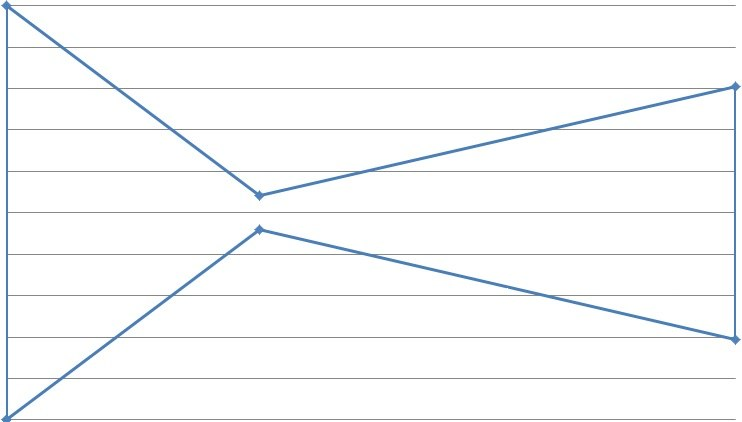
\includegraphics[width=5.7cm, height=3.4cm]{fon.jpg}};
\addplot [mark = none,line width = 0.05 cm, draw = red] coordinates{
( -0.059703 , 13999583 )
( -0.047762 , 13999086 )
( -0.035822 , 13997569 )
( -0.023881 , 13991101 )
( -0.011941 , 13938257 )
( 0.000000 , 8364175 )
( 0.023030 , 4566378 )
( 0.046060 , 1417927 )
( 0.069091 , 755822 )
( 0.092121 , 510240 )
( 0.115151 , 370466 )
( 0.138181 , 280970 )
( 0.161211 , 219938 )
( 0.184241 , 176461 )
( 0.207272 , 144434 )
( 0.230302 , 120197 )
( 0.253332 , 101440 )
( 0.276362 , 86647 )
( 0.299392 , 74788 )
( 0.322423 , 65146 )
( 0.345453 , 57209 )
};
\end{axis}
\end{tikzpicture}
\begin{flushright}
\textit{ Pic. $N^o 14$: Schedule changes in pressure on the projected profile of the nozzle } \\
\end{flushright}
\begin{tikzpicture}
\begin{axis} [
legend pos = outer north east,
height = 0.19\paperheight,
width = 0.4\paperwidth ]
\legend{  T };
\node[anchor=south west,inner sep=0] at (0,0) {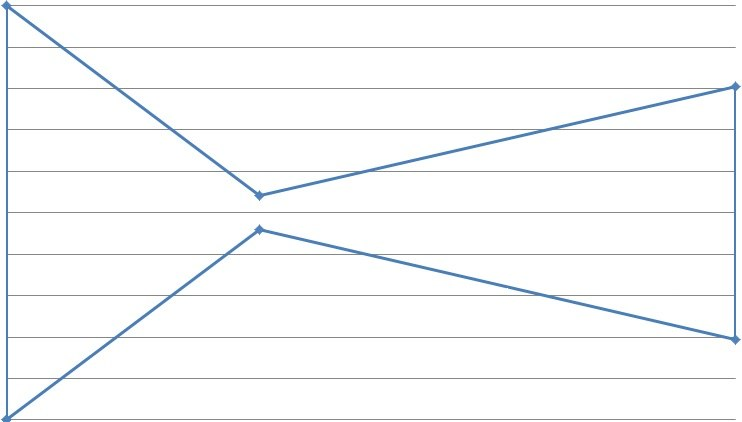
\includegraphics[width=5.7cm, height=3.4cm]{fon.jpg}};
\addplot[mark = none,line width = 0.05 cm, draw = red] coordinates {
( -0.059703 , 3199.982832 )
( -0.047762 , 3199.962342 )
( -0.035822 , 3199.899826 )
( -0.023881 , 3199.633123 )
( -0.011941 , 3197.450503 )
( 0.000000 , 2916.149283 )
( 0.023030 , 2614.630611 )
( 0.046060 , 2117.476387 )
( 0.069091 , 1890.370175 )
( 0.092121 , 1761.062719 )
( 0.115151 , 1662.281130 )
( 0.138181 , 1581.427114 )
( 0.161211 , 1513.107400 )
( 0.184241 , 1454.189283 )
( 0.207272 , 1402.607705 )
( 0.230302 , 1356.908306 )
( 0.253332 , 1316.022795 )
( 0.276362 , 1279.142272 )
( 0.299392 , 1245.639599 )
( 0.322423 , 1215.019098 )
( 0.345453 , 1186.882605 )
};
\end{axis}
\end{tikzpicture}
\begin{flushright}
\textit{ Pic. $N^o 15$: STemperature curve projected to the profile nozzle } \\
\end{flushright}
\begin{tikzpicture}
\begin{axis} [
legend pos = outer north east,
height = 0.19\paperheight,
width = 0.4\paperwidth ]
\legend{  v };
\node[anchor=south west,inner sep=0] at (0,0) {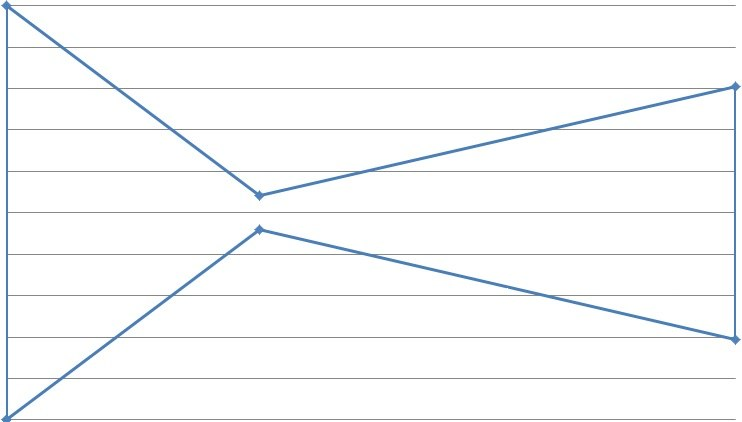
\includegraphics[width=5.7cm, height=3.4cm]{fon.jpg}};
\addplot[mark = none,line width = 0.05 cm, draw = red] coordinates {
( -0.059703 , 6.823497 )
( -0.047762 , 10.105979 )
( -0.035822 , 16.482674 )
( -0.023881 , 31.543460 )
( -0.011941 , 83.152703 )
( 0.000000 , 877.392913 )
( 0.023030 , 1259.981384 )
( 0.046060 , 1713.435708 )
( 0.069091 , 1884.618295 )
( 0.092121 , 1975.468262 )
( 0.115151 , 2042.149800 )
( 0.138181 , 2095.150644 )
( 0.161211 , 2138.911625 )
( 0.184241 , 2175.943939 )
( 0.207272 , 2207.855072 )
( 0.230302 , 2235.746684 )
( 0.253332 , 2260.408575 )
( 0.276362 , 2282.426094 )
( 0.299392 , 2302.244539 )
( 0.322423 , 2320.209981 )
( 0.345453 , 2336.596248 )
};
\end{axis}
\end{tikzpicture}
\begin{flushright}
\textit{ Pic. $N^o 16$: Schedule change the speed of the combustion products in the projected nozzle profile } \\
\end{flushright}
\begin{flushright}
\begin{scriptsize}
\textit{160700.65   Проектирование авиационных и ракетных двигателей\\
 Информационные технологии в АКТ: Лабораторный практикум} \\
\end{scriptsize}
\end{flushright}

\begin{large}
\textbf{\textit{Вывод по курсовой работе:}} Данная работа позволила овладеть навыками расчета на ПЭВМ параметров рабочих процессов двигателя с заданной начальной формой заряда. 

\begin{center}
\textbf{\textit{Литература :}}\\
\end{center}
1. Методические указания на курсовую работу по дисциплине 37528 “Информационные технологии в АКТ” – Кадомкин В.В. – М. 2014 г.
\begin{flushright}
Дата защиты курсовой работы: «04» июня 2015 г.\\
Подпись студента\rule{4cm}{0.01pt} \\
Подпись преподавателя\rule{4cm}{0.01pt} \\
\end{flushright}
\end{large}

\end{document}